Nous avons vu au chapitre précédent que les amas de galaxies pouvaient être utilisés comme une sonde cosmologique.
Nous avons également présenté les outils nécessaires pour pouvoir mener de telles études, et l'intérêt des suivis dédiés d'échantillons d'amas dans l'étalonnage de ces outils.

C'est dans ce contexte que s'inscrit le grand programme SZ de NIKA2, au sein duquel cette thèse s'est déroulée.
NIKA2 est une caméra permettant d'observer le ciel dans le domaine millimétrique avec une résolution angulaire bien meilleure que celle des instruments utilisés pour construire des catalogues d'amas.
L'instrument a été construit à Grenoble par la collaboration NIKA2, et choisie par l'Institut de Radioastronomie Millimétrique (IRAM) pour être un instrument résident de son télescope de 30 mètres.
En retour de la construction de NIKA2, la collaboration s'est vu attribuer un total de 1300 heures d'observations avec l'instrument.
Le grand programme SZ est l'un des programmes bénéficiant de ce temps garanti.

Dans ce chapitre, nous décrivons la caméra NIKA2 et le grand programme SZ.
Nous décrirons tout d'abord quelques éléments caractéristiques du télescope de 30 mètres de l'IRAM et de la caméra NIKA2.
Nous détaillerons ensuite l'utilisation de l'instrument, ses caractéristiques, puis le grand programme SZ, de son utilisation des capacités de NIKA2 à ses objectifs scientifiques.
La dernière section sera consacrée à la base de données du grand programme SZ, dont la création fait partie de ce travail de thèse.

% ===================================================================================== %
\section{Le télescope de 30 mètres de l'IRAM}\label{sec:30m}

% ------------------------------------------------------------------------------------- %
\subsection{Localisation et conditions météorologiques}\label{sec:30m_geo}

Le télescope de 30 mètres de l'Institut de Radioastronomie Millimétrique (IRAM, figure \ref{fig:30m}) est installé dans la chaîne de montagnes de la Sierra Nevada, proche de Grenade, dans le sud de l'Espagne \cite{baars_iram_1987}.
Il est situé à une altitude de près de 2900 mètres au dessus du niveau de la mer, proche du sommet Pico Veleta; ses coordonnées sont 03\textdegree23'58.1''W, 37\textdegree04'05.6''N.

\begin{figure*}[t]
    \centering
    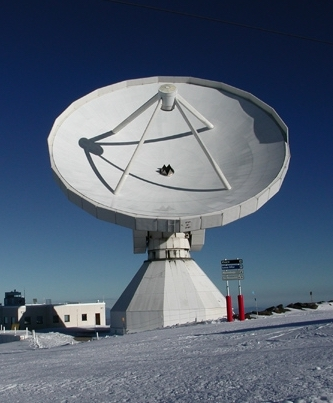
\includegraphics[height=7.5cm]{Figures/Chap_nk/30m_2.jpg}\hspace{10pt}
    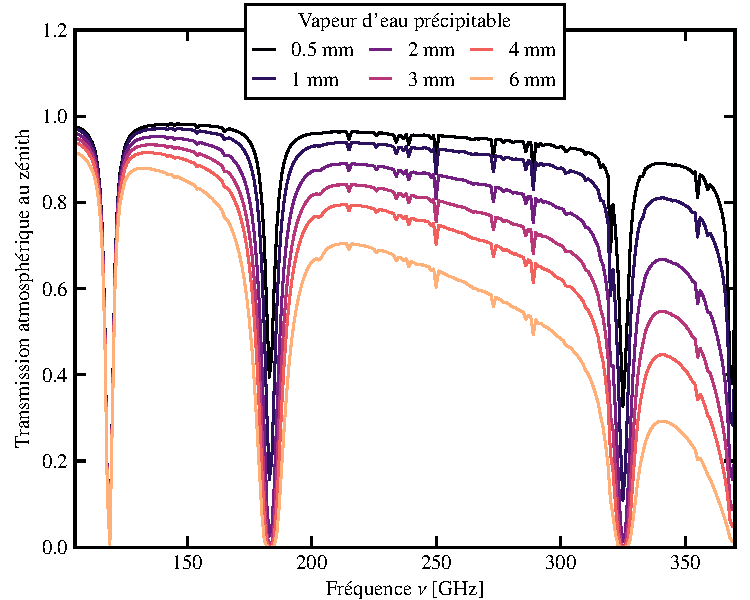
\includegraphics[height=7.5cm]{Figures/Chap_nk/atm_trans.pdf}
    \caption{
        \textbf{Gauche:} Photo du télescope de 30 mètres de l'IRAM.
        Crédit: \href{https://www.iram-institute.org/EN/photo-gallery.php?cat=2}{IRAM}.
        \textbf{Droite:} spectre de transmission atmosphérique en fonction de la quantité de vapeur d'eau précipitable, d'après le modèle de \myciteauthor{pardo_atmospheric_2001}.
    }
    \label{fig:30m}
\end{figure*}

Comme nous le verrons au chapitre suivant, l'une des sources de bruit principales dans les observations millimétriques est l'atmosphère.
Le bruit atmosphérique est principalement dû à son humidité.
Le site de Pico Veleta a donc été choisi pour son altitude, diminuant l'épaisseur de l'atmosphère traversée par les photons avant d'atteindre le télescope, mais également pour ses conditions météorologiques, en particulier son faible taux d'humidité.
Le spectre de transmission de l'atmosphère, calculé à l'aide du modèle de \myciteauthor{pardo_atmospheric_2001}, est représenté pour différentes valeurs de vapeur d'eau précipitable, correspondant à la quantité d'eau présente dans l'atmosphère.
On peut voir que pour des fréquences entre $100$ et $300$ GHz, la transmission est modulée par un continuum, dont la transmission diminue avec l'humidité, et par la présence de raies d'absorption (du dioxygène à $\sim 118$ GHz et de l'eau à $\sim 185$ et $325$ GHz).
Ces raies délimitent les gammes de longueurs d'onde observables depuis le sol, nommées fenêtres d'observation, centrées autour de $90$, $150$, $250$, et $350$ GHz.

En moyenne, les valeurs typiques de vapeur d'eau précipitable au télescope de 30 mètres sont de 7 mm en été, et de 3 mm en hiver.
En effet, la température de l'atmosphère est plus élevée l'été, augmentant la valeur de pression de vapeur saturante et donc la quantité d'eau qu'elle peut contenir.
Le télescope suit l'évolution de la quantité d'eau en temps réel en mesurant l'opacité atmosphérique au zénith $\tau_\nu$ grâce à un instrument résident dit taumètre, définie de façon à ce que la transmission de l'atmosphère $T_\nu$ à une fréquence $\nu$ soit
\begin{equation}
    \label{eq:tau_trans}
    T_\nu = \exp(- \tau_\nu / \sin(el)),
\end{equation}
où $el$ est l'élévation de l'objet observé. \\
L'opacité usuellement mesurée est $\tau_{225}$, à une fréquence de $225$ GHz, et vaut en moyenne $0.2$ en hiver et $0.5$ en été au télescope de 30 mètres.

La partie du ciel observable par le télescope est limitée au nord de la sphère céleste.
En effet, les objets de déclinaison inférieure à -20\textdegree\ en coordonnées équatoriales n'y atteignent jamais des élévations supérieures à 30\textdegree.
À de telles élévations, la couche d'atmosphère traversée par les rayons incidents est épaisse, et le poids du télescope commence à nuire à sa précision de pointage et affecter la forme de son lobe.
Les déclinaisons inférieures à -20\textdegree\ sont donc considérées comme inaccessibles pour le télescope.
Cela empêche l'observation d'amas découverts dans certaines régions des relevés réalisés dans l'hémisphère sud.
Comme le montre la figure \ref{fig:30m_sky}, une conséquence notable est l'impossibilité d'utiliser le télescope de 30 mètres pour le suivis d'amas des catalogues SPT \cite{bleem_galaxy_2015,bleem_sptpol_2020}, de même qu'environ la moitié du catalogue ACT \cite{hilton_atacama_2021}.
C'est la raison pour laquelle les amas de galaxies suivis par le grand programme SZ de NIKA2\footnote{Voir section \mypageref{sec:lpsz}} sont principalement issus du catalogue \textit{Planck}, couvrant tout le ciel, et de quelques uns des amas les plus au nord du catalogue ACT.

\begin{figure*}[t]
    \centering
    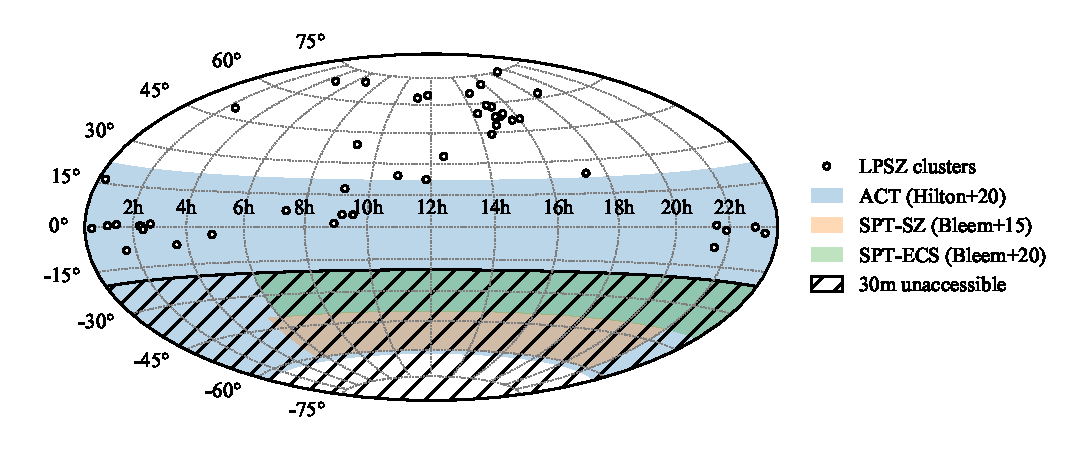
\includegraphics[width=.9\linewidth]{Figures/Chap_nk/footprints.pdf}
    \caption{
        Couvertures spatiales des relevés ACT (bleu, \cite{hilton_atacama_2021}) et SPT (orange et vert \cite{bleem_galaxy_2015,bleem_sptpol_2020}) en coordonnées équatoriales.
        Les axes horizontaux et verticaux représentent respectivement l'ascension droite et la déclinaison.
        La région hachurée marque les déclinaisons inaccessibles par le télescope de 30 mètres de l'IRAM.
        Les points représentent les coordonnées des amas du grand programme SZ de NIKA2 (voir section \ref{sec:lpsz} page \pageref{sec:lpsz}).
    }
    \label{fig:30m_sky}
\end{figure*}

% ------------------------------------------------------------------------------------- %
\subsection{Caractéristiques instrumentales}\label{sec:30m_opt}

Le télescope est constitué d'un miroir primaire paraboloïde de 30 mètres de diamètre, composé de panneaux d'aluminium et de polyuréthane \cite{baars_iram_1987}.
Afin de minimiser les variations de température induites par le lever et le coucher du soleil, qui entrainent une déformation du miroir primaire, ce dernier est activement thermalisé \cite{baars_thermal_1988} et peint de manière à réfléchir le rayonnement infrarouge.
Le miroir secondaire de 2 mètres de diamètre est maintenu à une distance de 10.5 mètres du primaire, égale à la distance focale de ce dernier.
L'ensemble est couplé à une cabine Nasmyth et installé sur une monture alt-azimuthale, pour une masse totale d'environ 800 tonnes.
Le télescope est présenté en figure \ref{fig:30m}.

Les rayons lumineux arrivent donc sur le miroir primaire du télescope, sont réfléchis par celui-ci vers le miroir secondaire, qui à son tour les redirige vers le vertex au centre du miroir primaire par lequel les faisceaux pénètrent dans la cabine.
La réponse angulaire du télescope, nommée \textit{lobe instrumental}, décrit la distribution du signal optique attendu à la sortie de ce vertex.
Dans le cas d'un signal monochromatique issu d'une source ponctuelle, cette réponse angulaire est donnée par la tâche d'Airy du miroir primaire à travers l'ouverture du vertex.
La largeur de celle-ci, déterminée par la largeur à mi-hauteur du pic principal, vaut $\theta = {\rm arcsin}(1.029 \times \lambda / D) =$ 14.1 et 8.2 arcsec pour des rayonnements monochromatiques de fréquences 150 et 260 GHz respectivement.
En pratique, le rayonnement incident est polychromatique, et ses multiples réflexions induisent un élargissement du lobe.
C'est la raison pour laquelle les différents instruments récepteurs dans la cabine du télescope ont des résolutions angulaires effectives moins bonnes que ces valeurs.

% ===================================================================================== %
\section{La caméra NIKA2}

La caméra NIKA2 (\textit{New IRAM KID arrays 2}) constitue l'instrument principal utilisé au cours de cette thèse.
Elle a été conçue par la collaboration internationale NIKA2, centrée à Grenoble, dans l'objectif de répondre à un appel d'offre de l'IRAM pour un nouvel instrument résident au télescope de 30 mètres.
Dans cette section, nous présentons brièvement l'instrument et son fonctionnement.
Plus de détails peuvent être trouvés dans \cite{adam_nika2_2018,perotto_calibration_2020}.
% ------------------------------------------------------------------------------------- %
\subsection{Détecteurs à inductance cinétique}\label{sec:kids}

Les détecteurs utilisés par NIKA2 sont des détecteurs à inductance cinétique (KID, pour \textit{kinetic indictance detectors}, \cite{day_broadband_2003,roesch_development_2012}).
Leur utilisation est l'une des spécificités de NIKA2, puisque la plupart des instruments millimétriques utilisent des détecteurs bolométriques.

Les KID sont des détecteurs supraconducteurs.
Ils sont constitués d'un matériau caractérisé par une température critique $T_c$ en dessous de laquelle les électrons sont séparés en deux populations: d'une part, des électrons appariés en \textit{paires de Cooper}, et d'autre part des électrons libres, nommés \textit{quasi-particules}.
La densité de paires de Cooper $n_s$ est alors donnée en fonction de la température $T$ par \cite{gorter_supraconductivity_1934}:
\begin{equation}
    \label{eq:cooper_dens}
    \frac{n_s}{n} = 1 - \left(\frac{T}{T_c}\right)^4,
\end{equation}
où $n$ est la densité totale des porteurs de charges, quasi-particules et paires de Cooper. \\
Les paires de Cooper forment des condensats de Bose-Einstein, pouvant être brisée par une énergie dite de \textit{gap}, notée $2\Delta$, et pouvant être calculée dans le cadre de la théorie Bardeen-Cooper-Schrieffer \cite{bardeen_microscopic_1957,bardeen_theory_1957} comme:
\begin{equation}
    2\Delta \simeq 3.53 \, k_\textsc{b} T_c.
\end{equation}
D'après l'équation (\ref{eq:cooper_dens}), pour des températures $T \ll T_c$, la majorité des charges est donc portée par des paires de Cooper ($n_s \simeq n$).
Alors, des photons incidents d'énergie supérieure au \textit{gap} $2\Delta$ pourront briser ces paires et changer la distribution des porteurs de charges entre paires de Cooper et quasi-particules.

Lorsqu'un supraconducteur est traversé par un courant électrique, la conduction peut être assurée par chacun des porteurs de charges.
Dans le cas d'un courant alternatif cependant, les paires de Cooper sont sujettes à une inertie, qui freine leur mouvement, et s'oppose donc à la conduction.
Ce phénomène crée une inductance qualifiée de cinétique $L_k$ dans le matériau, dont l'impédance s'écrit alors $Z = R_{qp} + i\omega L_k$, où $R_{qp}$ est la résistance liée aux quasi-particules, et $\omega$ la pulsation du courant alternatif.
Il apparaît naturellement qu'une variation de densité de paires de Cooper, par brisure de certaines d'entre elles par des photons incidents, créera une variation d'inductance cinétique $\delta L_k$.
Celle-ci est inversement proportionnelle à la variation de densité de paires de Cooper, et donc proportionnelle à la variation de puissance optique incidente (voir par exemple \cite{day_broadband_2003} pour une démonstration).

Le fonctionnement des KID est basé sur la mesure de variation de fréquence de résonance induite par un changement de puissance optique reçue.
Les détecteurs de NIKA2 sont des détecteurs à inductance de type LEKID (\textit{Lumped Element KID}, \cite{roesch_development_2012}).
Chaque KID est un circuit résonant de type RLC, constitué d'une partie capacitive $C$, d'un méandre inductif servant d'absorbeur de flux, d'inductance géométrique $L_g$ s'ajoutant à l'inductance cinétique $L_k$, et d'une résistance $R$.
La fréquence de résonance d'un KID est donc donnée par:
\begin{equation}
    \label{eq:kids_freq}
    f = \frac{1}{2\pi \sqrt{(L_g + L_k)C}}.
\end{equation}
Ainsi, une variation de puissance optique incidente sur le détecteur va induire un changement de la proportion de porteurs de charges sous forme de paires de Cooper, ce qui créera une variation de l'inductance cinétique du supraconducteur, qui aura à son tour pour conséquence une modification de la fréquence de résonance du détecteur.
La dérivation de l'équation (\ref{eq:kids_freq}) par rapport à l'inductance cinétique $L_k$ permet d'exprimer cette variation de fréquence de résonance par rapport au changement d'inductance cinétique:
\begin{equation}
    \delta f = \pdv{f}{L_k} \delta L_k = -2 \pi^2 C \, f^{\;3} \delta L_k.
\end{equation}
Comme nous l'avons vu précédemment, le changement d'inductance cinétique est inversement proportionnel à la variation de puissance optique incidente; ainsi,
\begin{equation}
    \delta f \propto \delta L_k \propto -\delta P_{\rm opt}.
\end{equation}

La mesure de cette variation de fréquence de résonance permet donc de remonter à la variation de puissance optique l'ayant causée.
Afin de mesurer $\delta f$, les détecteurs sont couplés à des lignes de transmission, parcourues par un signal alternatif.
Celles-ci sont couplées inductivement aux méandres des KID: le signal transmis est donc affecté par la présence de chaque détecteur.
La variation en phase et en amplitude du signal de la ligne de transmission due à la présence d'un KID est liée à la fréquence de résonance de ce dernier.
Ainsi, la mesure de la phase et de l'amplitude du signal de sortie de la ligne de lecture permet de reconstruire la variation de fréquence de résonance des détecteurs présents le long de cette ligne, et \textit{in fine} à la variation de puissance lumineuse.

Comme le montre l'équation (\ref{eq:kids_freq}), la fréquence de résonance d'un KID est liée à la capacité de son condenseur $C$.
Ainsi, la fréquence de résonance de chaque détecteur peut être ajustée par contrôle des des propriétés géométriques du condenseur.
Cette caractéristique fait des KID des détecteurs intrinsèquement adaptés au multiplexage: un grand nombre de détecteurs peuvent avoir des fréquences de résonance différentes et être montés sur une même ligne de lecture.
Par conséquent, la quantité de câbles électroniques nécessaires à la transmission des signaux d'une matrice de détecteurs est fortement diminuée par rapport aux bolomètres, nécessitant une ligne de lecture par détecteur.
Au vu des contraintes cryogéniques importantes pour les détecteurs, une augmentation du nombre de détecteurs lisibles par une ligne de lecture permet l'augmentation du nombre de détecteurs sans pour autant augmenter le nombre de câbles devant sortir du cryostat.
Cette qualité fait des KID des détecteurs particulièrement compétitifs.

Un des KID de la caméra NIKA et une matrice de détecteurs installée dans NIKA2 sont présentés en figure \ref{fig:nk_kids}.
Le panneau de gauche montre les différentes parties du détecteur: le condensateur (en haut), et le méandre inductif, occupant la majorité de la surface du détecteur et dans lequel les photons sont absorbés et peuvent briser des paires de Cooper.
On voit également la ligne de transmission utilisée pour lire le détecteur qui en longe le côté inférieur.
Sur le panneau droit, on voit une des matrices de 1140 KID de NIKA2.
Les détecteurs individuels ne sont pas distinguables, mais on peut voir les huit lignes de transmission utilisées pour la lecture des 1140 détecteurs.

\begin{figure*}[t]
    \centering
    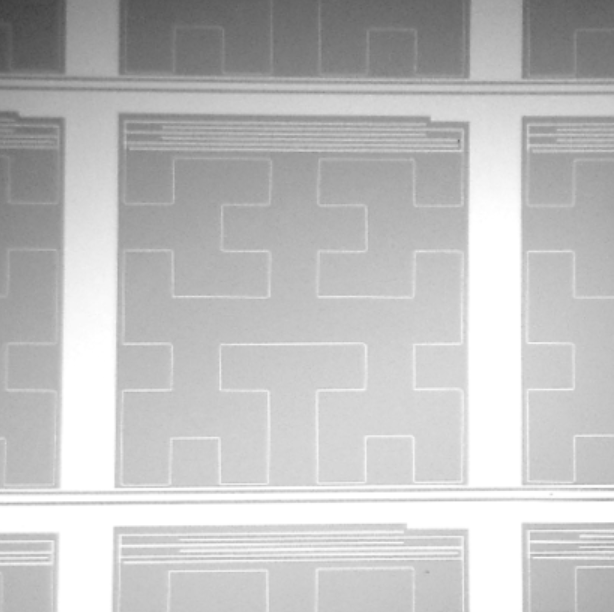
\includegraphics[height=7cm]{Figures/Chap_nk/fig3_AB.png}
    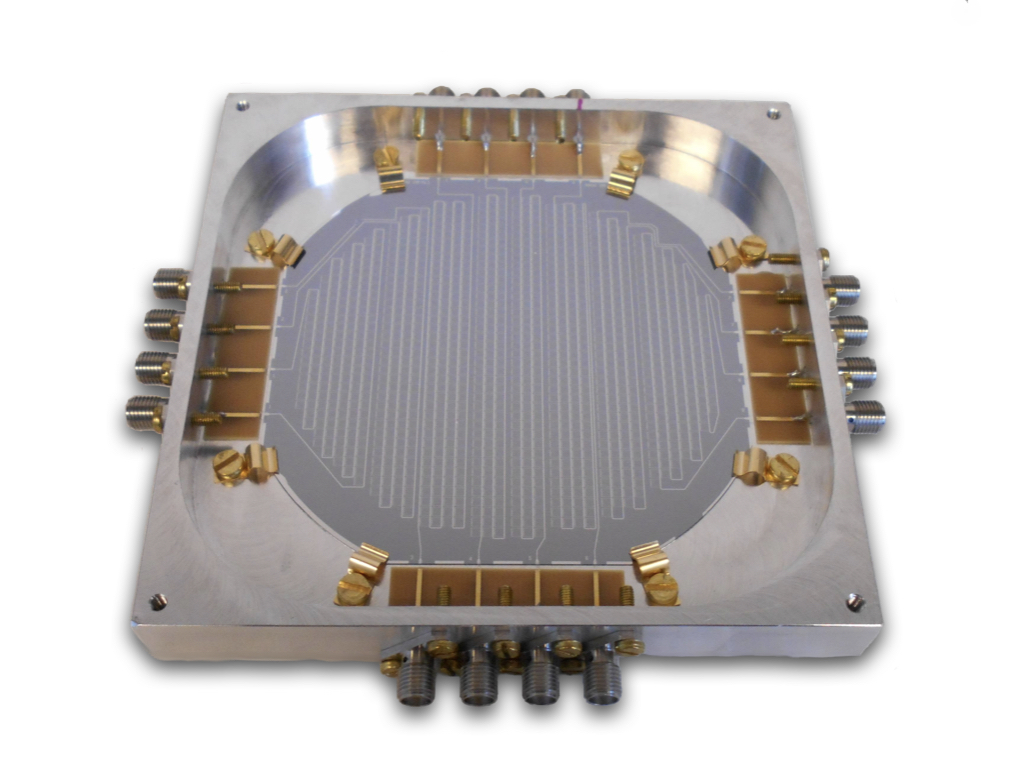
\includegraphics[height=7cm]{Figures/Chap_nk/1mm_array.jpeg}
    \caption{
        \textbf{Gauche:} Image d'un détecteur KID de NIKA, de taille 2.3 mm $\times$ 2.3 mm.
        Le méandre inductif du détecteur couvre la plupart de sa surface, tandis que la partie capacitive $C$ est située dans la partie haut du détecteur.
        \textbf{Droite:} Matrice de KID dans la bande à 260 GHz de NIKA2, comportant 1140 KID et 8 lignes de transmission.
        Figures extraites de \cite{adam_nika2_2018}.
    }
    \label{fig:nk_kids}
\end{figure*}


% ------------------------------------------------------------------------------------- %
\subsection{Éléments clés de la caméra NIKA2}

Les KID de NIKA2 sont constitués d'une couche mince d'aluminium d'environ 18 nm d'épaisseur.
La température critique de l'aluminium étant de $T_c = 1.19 \;\unit{K}$, l'énergie du \textit{gap} vaut $2\Delta \simeq 0.36 \;\unit{meV}$, correspondant à des photons à une fréquence de l'ordre de 90 GHz.
De tels détecteurs sont donc tout à fait appropriés pour la mesure du fond diffus cosmologique et de l'effet SZ (cf. figure \ref{fig:tsz_spec}).

La caméra NIKA2 est dotée de trois matrices de KID.
Deux matrices (A1 et A3), chacune composée de 1140 détecteurs, sont placées derrière une lame dichroïque transmettant une gamme de fréquence centrée à 260 GHz.
La troisième (A2) est quant à elle dédiée à l'observation de photons de fréquence autour de 150 GHz.
Les deux bandes passantes de NIKA2 sont donc adaptées aux fenêtres d'observation disponibles au vu de la transmission atmosphérique (cf. figure \ref{fig:30m}).
Elles sont illustrées sur la figure \ref{fig:nk_bp}.
Il y apparait que les bandes passantes de NIKA2 exploitent parfaitement les fenêtres spectrales disponibles pour des observations millimétriques depuis le sol, de même que la dépendance spectrale de l'effet Sunyaev-Zeldovich, avec une bande de chaque côté du zéro de la distorsion spectrale (cf. section \ref{sec:sz}).
Ce point sera abordé plus en détail en \mypageref{sec:lpsz}.

\begin{figure*}[t]
    \centering
    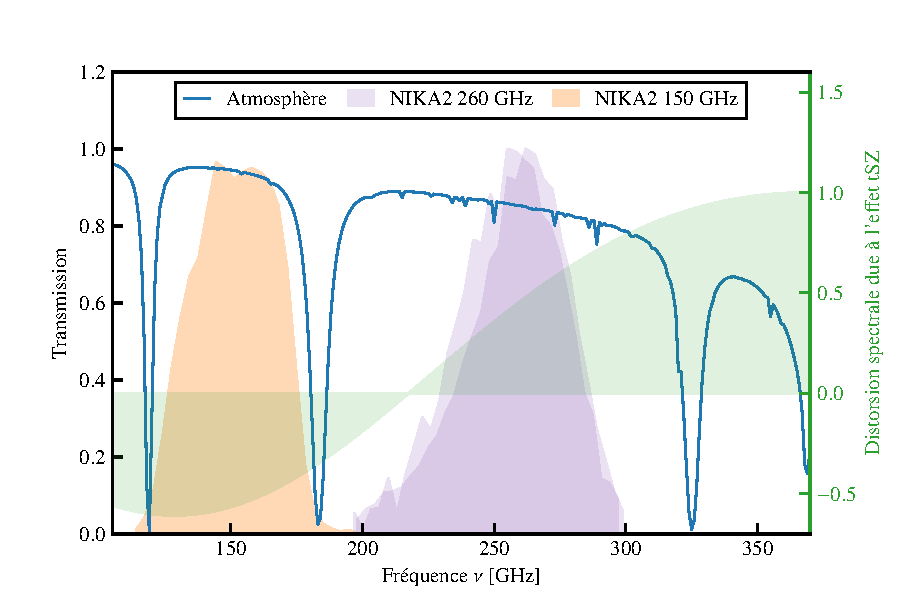
\includegraphics[width=.8\linewidth]{Figures/Chap_nk/bandpasses.pdf}
    \caption{
        Bandes passantes de NIKA2 à 260 GHz (violet) et 150 GHz (orange).
        La transmission atmosphérique calculée à partir du modèle de \myciteauthor{pardo_atmospheric_2001} pour 2 mm de vapeur d'eau précipitable est également représentée en bleu.
        La distorsion spectrale due à l'effet tSZ est montrée en vert.
    }
    \label{fig:nk_bp}
\end{figure*}

Comme nous l'avons discuté en \ref{sec:kids}, le fonctionnement des détecteurs à inductance cinétique requiert que ceux-ci soient refroidis à une température inférieure à leur température critique.
Dans le cas de NIKA2, cette condition est assurée par un cryostat, maintenant les détecteurs à une température d'environ 150 mK, bien en deçà de la température critique de l'aluminium.

Un système optique dévie les rayons lumineux focalisés par le télescope (cf. section \ref{sec:30m_opt}) vers les matrices de KID.
Celui-ci est tout d'abord composé de quatre miroirs dans la cabine du télescope, dirigeant les rayons issus du miroir secondaire du télescope vers le cryostat de NIKA2.
Une fois qu'ils ont pénétré le cryostat, les rayons lumineux sont réfléchis par une succession de miroirs refroidis, puis traversent un filtre dichroïque, séparant la lumière en deux.
Celui-ci permet de diriger une partie des rayons incidents vers la matrice de KID à 150 GHz, et l'autre vers les matrices à 260 GHz.
La présence des deux matrices à 260 GHz et d'un élément polariseur permet à NIKA2 d'être sensible à la polarisation des photons incidents à 260 GHz.
Dans le travail développé au cours de cette thèse, cette capacité ne sera pas exploitée, et les données issues des deux matrices à 260 GHz sont combinées en une unique carte du ciel à cette fréquence.

% ===================================================================================== %
\section{Observations avec NIKA2} \label{sec:nk_obs}

Les observations avec la caméra NIKA2 réalisées et étudiées au cours de cette thèse suivent une procédure précise, dont le but est la production de cartes fidèles du ciel.
Dans cette section, nous détaillons cette procédure, ainsi que les performances de l'instrument.
L'étape suivante, visant à isoler les signaux astrophysiques des différents contaminants, sera détaillée au chapitre suivant.

% ------------------------------------------------------------------------------------- %
\subsection{Balayage du ciel et données ordonnées en temps} \label{sec:nk_otf_toi}

Comme nous l'avons vu dans la section précédente, les KID permettent de mesurer une variation de puissance lumineuse.
Ainsi, ils sont moins adaptés à la mesure de signaux stationnaires qu'à celle de signaux variant dans le temps.
Pour pouvoir mesurer des signaux stationnaires, tels que les signaux astrophysiques étudiés au cours de cette thèse, il est donc nécessaire d'adopter une stratégie visant à moduler le signal d'intérêt dans le temps.

Dans le cas de NIKA2, cet objectif est accompli en balayant le ciel par des \textit{scans}, dont le principe est le suivant.
Le télescope se déplace suivant une trajectoire déterminée, de sorte à ce que la position sur le ciel d'un détecteur de référence soit connue à tout instant.
Chacun des KID de NIKA2 enregistre alors la variation de la puissance lumineuse qu'il reçoit au cours du temps.
Les données enregistrées sont par conséquent ordonnées en temps, et nommées TOI pour \textit{Time Ordered Information}.
Une fois le balayage terminé, une matrice de pointage est calculée, donnant la position de chaque KID sur le ciel au cours du temps à partir du pointage de référence du télescope et de la position relative de chaque KID par rapport à ce centre de référence (la mesure de celle-ci sera détaillée en \ref{sec:focal_plane_reconstruction}).
La matrice de pointage permet alors de projeter les TOIs de chaque KID en cartes du ciel.
En plus de moduler temporellement le signal pour le rendre détectable par les KID, cette méthode permet d'exploiter la redondance du signal et les corrélations entres les différentes sources de bruit.
Comme nous le verrons au chapitre suivant, cette redondance facilite la différenciation du signal et du bruit dans les données.

\begin{figure*}[t]
    \centering
    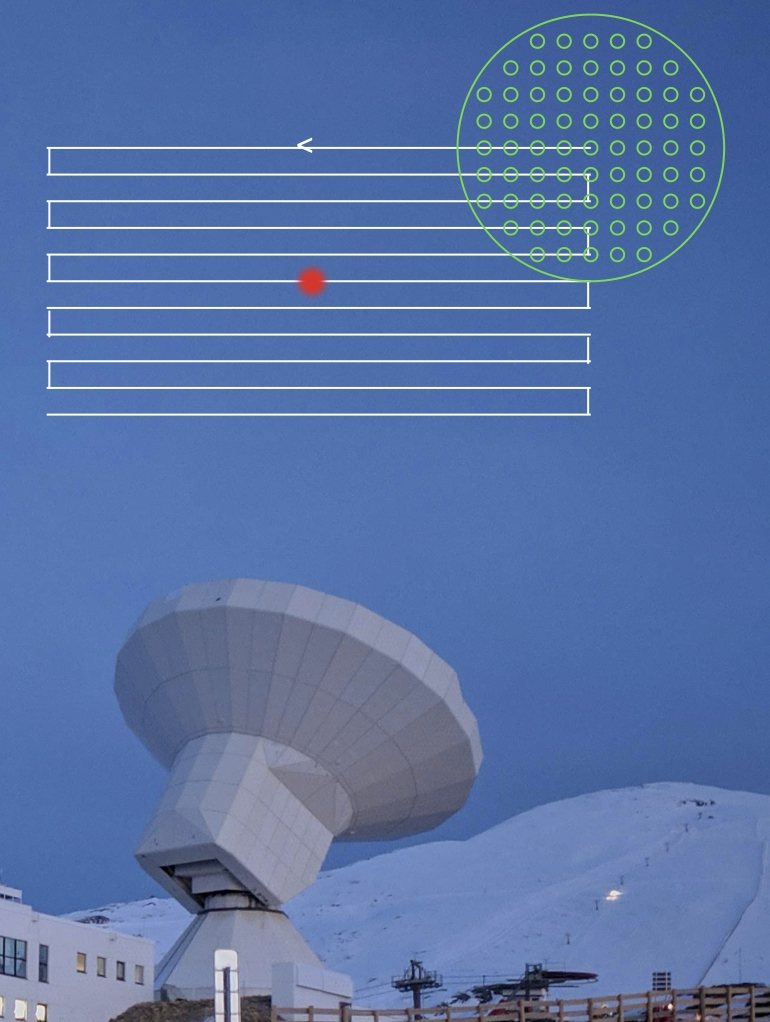
\includegraphics[height=8cm]{Figures/Chap_nk/otf_telescope_source.jpg}\hspace{10pt}
    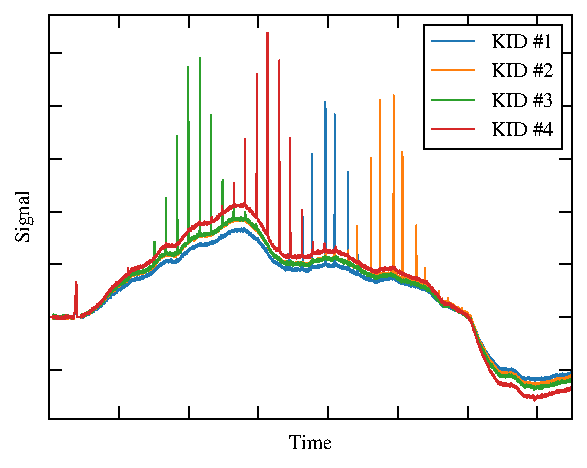
\includegraphics[height=7.5cm]{Figures/Chap_nk/tois.pdf}
    \caption{
        \textbf{Gauche:} illustration du mouvement effectué par le télescope dans le ciel (en blanc) lors d'un scan OTF.
        La matrice de détecteurs est représentée en vert, et la source observée en rouge.
        \textbf{Droite:} représentation des données ordonnées en temps obtenues par scan d'Uranus pour trois KID.
        La détection de la source se manifeste par un pic de signal détecté.
    }
    \label{fig:nk_otf_toi}
\end{figure*}

La trajectoire suivie par le télescope pour réaliser un scan est nommée stratégie de scan.
Le choix de celle-ci est capital, puisqu'il a un grand impact sur la capacité à reconstruire le signal astrophysique (comme nous le verrons dans le chapitre suivant).
Dans le cas des observations de l'effet SZ discutées au cours de cette thèse, la stratégie employée est basée sur la réalisation de scans OTF (pour \textit{on the fly}): une successions de \textit{subscans} rectilignes parallèles en coordonnées équatoriales sont effectués, espacés d'un pas constant.
Cette stratégie induit un mouvement du télescope en forme de serpentin, illustrée sur le panneau gauche de la figure \ref{fig:nk_otf_toi}.
Les données ordonnées en temps obtenues pour un tel \textit{scan} sur une source ponctuelle brillante (Uranus) sont représentées sur le panneau droit de la figure \ref{fig:nk_otf_toi}.
Étant données les différentes positions des détecteurs dans le plan focal, ces derniers ne détectent pas le passage de la source au même moment, ce qui se manifeste par un décalage en temps du signal de la source.
Les observations du grand programme SZ sont effectuées par groupes de quatre scans, à des angles de $0^\circ$, $45^\circ$, $90^\circ$, et $135^\circ$ par rapport à l'axe des ascensions droites, afin de maximiser l'isotropie de la couverture du ciel.
Ce point sera discuté plus en détail au chapitre suivant.

% ------------------------------------------------------------------------------------- %
\subsection{Reconstruction du plan focal}\label{sec:focal_plane_reconstruction}

Le grand nombre de détecteurs présents sur une même ligne de lecture peut causer des difficultés à isoler les signaux provenant de chaque détecteur.
En particulier, la lecture de la fréquence de résonance d'un détecteur ne permet pas de connaître sa position dans la matrice.
De plus, la fréquence de résonance de certains détecteurs peut ne pas être trouvée, ou bien être trop proche de celle d'un détecteur voisin, auquel cas les signaux en provenance des deux KID sont incorrectement associés à un seul détecteur.
Il est donc nécessaire, avant d'observer, de reconstruire le plan focal de la caméra en associant chaque fréquence de résonance à un KID, permettant de connaître sa position et d'identifier les détecteurs invalides.

Pour cela, une carte profonde d'une source brillante, par exemple une planète comme Uranus, est réalisée de façon à ce qu'une carte de la source puisse être construite pour chaque détecteur.
Ces cartes, nommées \textit{beammaps}, ont plusieurs vertus.
Elles permettent d'une part, pour chaque détecteur, de connaître sa position dans la matrice par rapport à un KID de référence, ce qui permettra la reconstruction des observations du ciel détaillée par la suite.
Elles permettent également l'identification des détecteurs en diaphonie, pour lesquels deux sources apparaissent sur une même carte, de même que les détecteurs hors résonance.
Les gains des KID, quantifiant l'étalonnage relatif de chaque détecteur, sont également calculés à partir de ces cartes grâce au rapport entre le flux connu de la source et la variation de fréquence de résonance correspondante pour chaque détecteur.
Enfin, ces cartes sont utilisées pour la mesure du lobe instrumental observé par chacun des détecteurs, discutée en \mypageref{sec:nk_perf}.

% ------------------------------------------------------------------------------------- %
\subsection{Pointage et focalisation}\label{sec:pointing_focus}

Avant d'observer des sources, il est nécessaire de s'assurer que le télescope est à même de livrer des observations fidèles du ciel.
Il faut donc s'assurer que le KID de référence est correctement aligné avec l'axe optique du télescope, et que ce dernier est correctement focalisé.

Le pointage du télescope est vérifié en réalisant un mouvement d'aller-retour sur une source, tout d'abord en azimut, puis en élévation, formant une croix dans le plan du ciel.
Des profils Gaussiens sont ajustés sur les TOIs d'un détecteur de référence au centre des matrices de NIKA2.
La position de la source dans le ciel étant connue, il est alors possible d'associer des coordonnées célestes au détecteur de référence, et par extension aux autres KID des matrices de NIKA2.
Un exemple de procédure de pointage est présenté en figure \ref{fig:nk_pointing}, illustrant la carte obtenue pour un pointage sur Uranus.
L'ajustement des profils de la source le long des axes des azimuts et élévations mesurés par le détecteur de référence (bas de la figure) permet de faire correspondre les coordonnées de chacun des détecteurs dans le plan focal avec ses coordonnées célestes\footnote{Notons que la procédure utilisée pour le pointage ajuste le profil de la source sur les TOI du KID de référence, alors que les profils représentés sur la figure \ref{fig:nk_pointing} sont ceux de la carte déjà projetée.}.

\begin{figure*}[t]
    \centering
    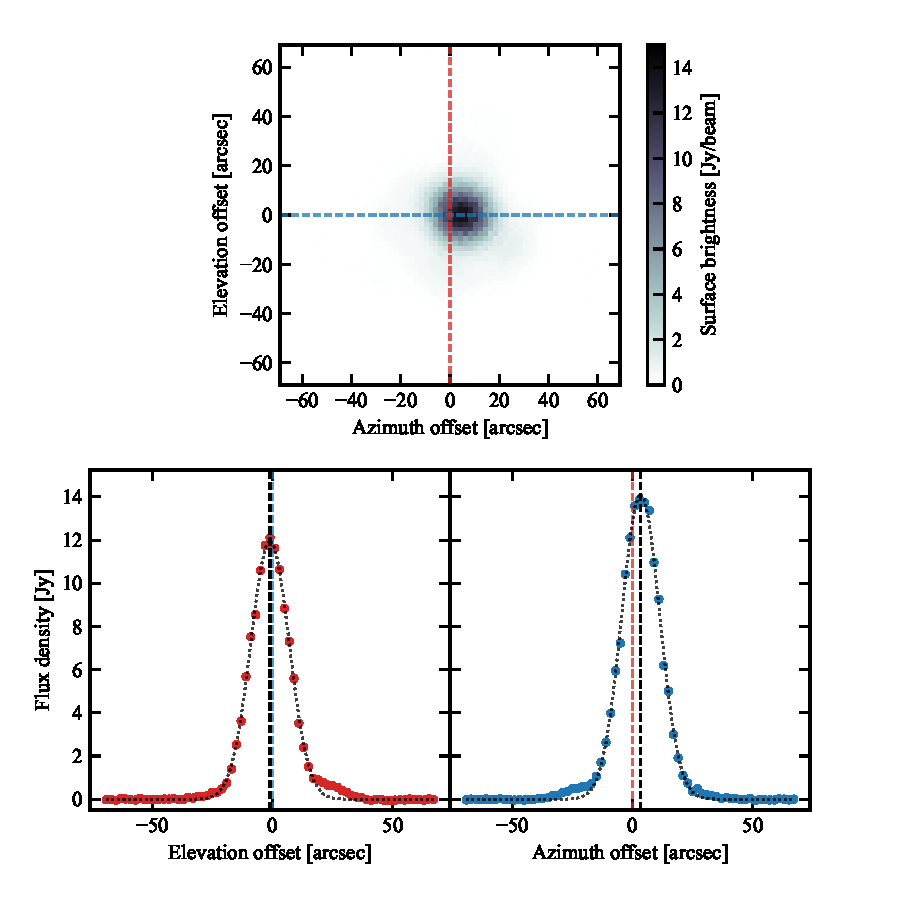
\includegraphics[width=.8\linewidth]{Figures/Chap_nk/pointing.pdf}
    \caption{
        Exemple de procédure de pointage.
        \textbf{Haut:} carte d'Uranus obtenue avec un scan en croix, suivant les directions des lignes bleue puis rouge, projetée en utilisant la matrice de pointage avant correction de pointage.
        \textbf{Bas:} profils de la planète le long de l'axe des élévations (\textit{gauche}) et des azimuts (\textit{droite}).
        L'ajustement des profils par une gaussienne (courbes pointillées noires) permet de mesurer le centre de la source dans les deux directions (lignes noires verticales).
        La différence entre la position de la source et celle du centre de la carte donne les corrections de pointage utilisées pour réaligner le KID de référence.
    }
    \label{fig:nk_pointing}
\end{figure*}

La focalisation du télescope quantifie l'accord entre la position du miroir secondaire et le point focal du miroir primaire.
Lorsque le télescope est défocalisé, c'est-à-dire lorsque le miroir secondaire est éloigné du point focal du primaire, les rayons ne sont pas réfléchis correctement vers le système optique, induisant des déformations de l'image reconstruite avec NIKA2, et notamment un élargissement du lobe.
Il faut alors positionner correctement le miroir secondaire.
Afin de connaître la position optimale de celui-ci, un scan OTF est effectué sur une source brillante pour cinq distances différentes entre les miroirs primaire et secondaire, espacées de $0.4 \;\unit{mm}$.
Les cartes obtenues à partir de ces observations sont créées et utilisées pour ajuster un modèle de lobe gaussien.
La procédure est illustrée en figure \ref{fig:nk_focus} avec la matrice à 150 GHz de NIKA2.
Cinq cartes d'Uranus sont produites (haut) et ajustées avec un modèle de lobe gaussien, permettant de mesurer la largeur du lobe et le flux de la source pour chacune des cartes.
Ces résultats sont ajustés avec une loi parabolique, dont le maximum donne les valeurs de la distance primaire-secondaire maximisant le flux et minimisant la largeur du lobe.
L'une ou l'autre de ces deux distances peut être choisie comme distance optimale pour la focalisation du télescope, selon la qualité de l'ajustement.
On note que les résultats des deux estimateurs sont en général très proches -- une différence de 0.03 mm est trouvée dans l'exemple de la figure \ref{fig:nk_focus}.

Un pointage correct est important pour toutes les observations réalisées avec NIKA2, incluant les observations de l'effet SZ.
Un mauvais pointage entraîne une connaissance imprécise de la position des détecteurs, et empêche donc la construction de cartographies fidèles du ciel.
Une erreur systématique sur le pointage de toutes les observations d'une source entraîne une mauvaise reconstruction des coordonnées du signal dans le ciel, qui a pour conséquence l'impossibilité de comparer des cartes NIKA2 avec des données issues d'autres instruments.
Comme nous le verrons dans les chapitres \ref{chap:panco} et \ref{chap:actj0215}, de telles comparaisons sont au cœur des analyses du grand programme SZ traitées dans cette thèse, et sont nécessaires à l'étude des propriétés thermodynamiques des amas de galaxies et des contaminants astrophysiques.
D'autre part, des imprécisions régulières (par exemple, variant d'un scan à l'autre) entraîne une dilution du signal, l'attribuant à des positions incorrectes, et donc un élargissement effectif du lobe de l'instrument.
Comme nous le verrons en section \mypageref{sec:lpsz}, la résolution angulaire de NIKA2 est l'un de ses principaux atouts pour la mesure de l'effet SZ.
La précision du pointage pouvant être dégradée par les mouvements du télescope, celui-ci est vérifié régulièrement au cours des observations, environ une fois par heure.
De même, comme le montre la figure \ref{fig:nk_focus}, une mauvaise focalisation du télescope entraîne un élargissement du lobe, et donc une dégradation de la résolution angulaire.
La focalisation variant principalement avec la géométrie du miroir primaire, qui se déforme avec les changements de température.
C'est pour cette raison que les observations diurnes avec NIKA2 doivent éviter l'illumination du miroir primaire avec le soleil, et que la focalisation est vérifiée à intervalles réguliers (toutes les heures de jour, et toutes les deux à trois heures la nuit).

\begin{figure*}[t]
    \centering
    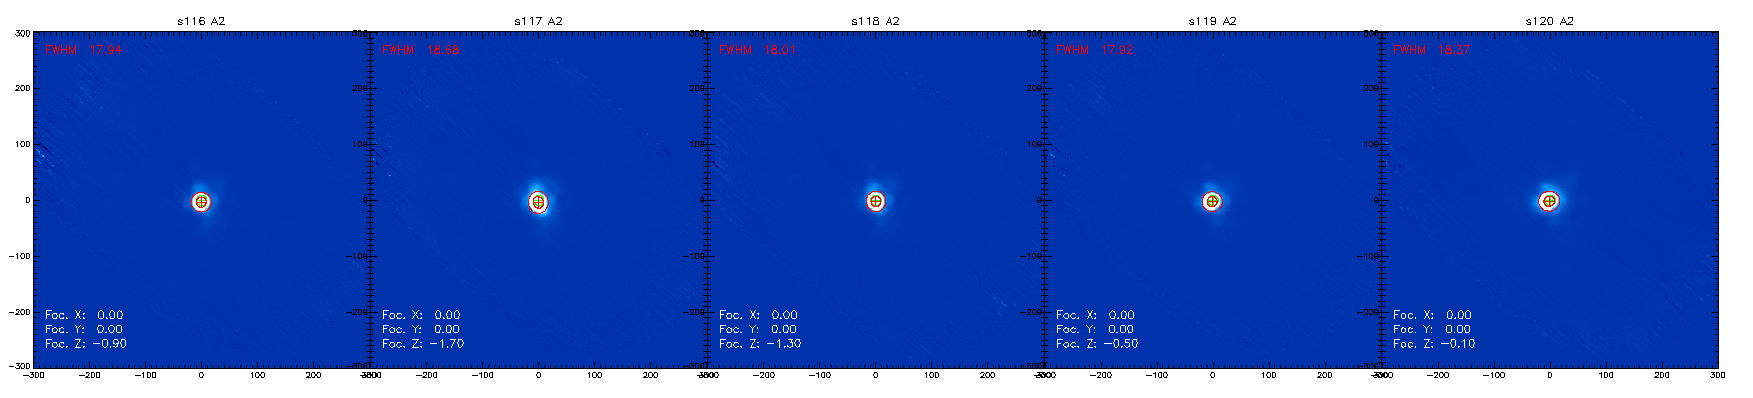
\includegraphics[width=.9\linewidth]{Figures/Chap_nk/focus_maps_crop.png}
    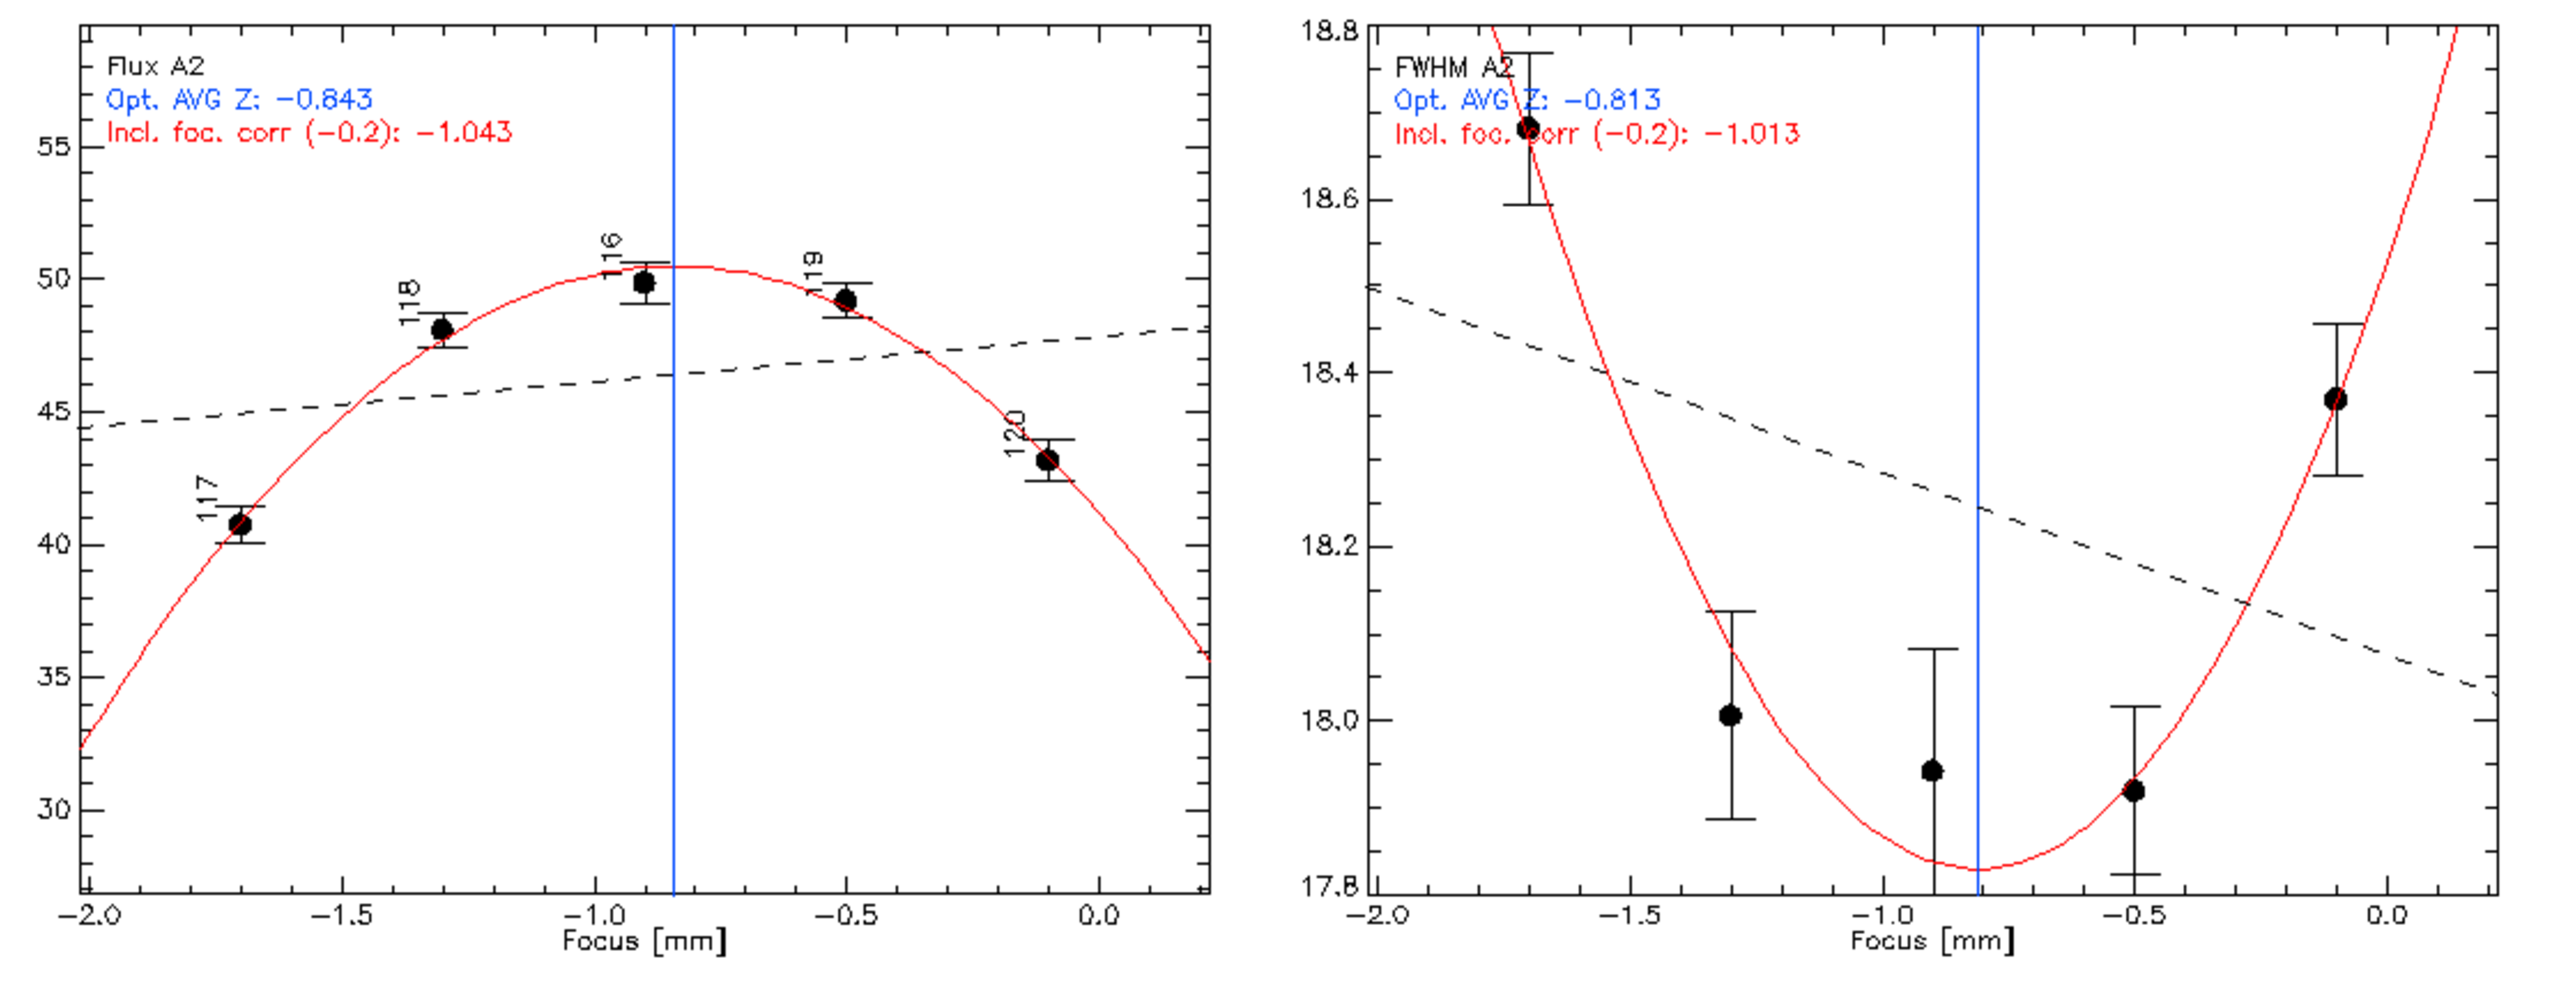
\includegraphics[width=.9\linewidth]{Figures/Chap_nk/focus_results_crop.pdf}
    \caption{
        Exemple de procédure de focalisation du télescope.
        \textbf{Haut:} cartes à 150 GHz d'Uranus obtenue pour cinq distances primaire-secondaire.
        \textbf{Bas:} Flux d'Uranus (\textit{gauche}) et largeur à mi-hauteur (\textit{droite}) mesurées dans chacune des cartes (noir).
        L'ajustement des points avec une loi parabolique (rouge) permet de mesurer la distance permettant une focalisation optimale du télescope (bleu).
    }
    \label{fig:nk_focus}
\end{figure*}

% ------------------------------------------------------------------------------------- %
\subsection{Performances instrumentales de NIKA2}\label{sec:nk_perf}

Les caractéristiques de NIKA2 ont été mesurées par la collaboration du même nom au cours de sa phase de \textit{commissioning}.
Ces mesures sont décrites avec un grand niveau de détail par \myciteauthor{perotto_calibration_2020}, et nous n'en donneront que les résultats principaux nécessaires à la description du travail effectué dans cette thèse.
La phase de \textit{commissioning} de l'instrument a eu lieu entre Octobre 2015 et Avril 2017.
Elle a permis de mesurer avec précision les caractéristiques de l'instrument, telles que son lobe et sa sensibilité.
La mesure des performances de l'instrument a quant à elle eu lieu au cours de trois campagnes d'observations en Février et Octobre 2017 et Janvier 2018.
Les résultats principaux de ces mesures sont consignés dans la table \ref{tab:nk_specs}, et nous détaillons ici brièvement la signification des caractéristiques et la méthode de calcul.

\begin{table}[t]
    \setlength{\tabcolsep}{15pt}
    \small
    \centering
    \begin{tabular}{l r r}
        \toprule
        Caractéristique & Matrices A1 et A3 & Matrice A2 \\
        \midrule
        \midrule
        \multicolumn{3}{c}{\itshape Bandes passantes} \\
        \midrule
        Longueur d'onde de référence [mm]   & 1.15 & 2.00 \\
        Fréquence de référence [GHz]        & 260  & 150  \\
        \midrule
        \multicolumn{3}{c}{\itshape Nombre de détecteurs} \\
        \midrule
        Nombre de détecteur présents        & $1140 \times 2$ & 616 \\
        Fraction de détecteurs valides [\%] & 84 & 90 \\
        \midrule
        \multicolumn{3}{c}{\itshape Résolution angulaire et champ de vue} \\
        \midrule
        Largeur à mi-hauteur (FWHM) du lobe principal [arcsec] & $11.1 \pm 0.2$ & $17.6 \pm 0.1$ \\
        Champ de vue instantané [arcmin]    & 6.5 & 6.5 \\
        \midrule
        \multicolumn{3}{c}{\itshape Incertitudes de pointage et d'étalonnage} \\
        \midrule
        Erreurs de pointage [arcsec] & $<3$ & $<3$ \\
        Incertitude sur l'étalonnage absolu [\%] & 5 & 5 \\
        Incertitude RMS sur l'étalonnage de sources ponctuelles [\%] & 5.7 & 3.0 \\
        \midrule
        \multicolumn{3}{c}{\itshape Sensibilité} \\
        \midrule
        NEFD [$\unit{mJy \cdot s^{1/2}}$]  & $30 \pm 3$ & $9 \pm 1$ \\
        \textit{Mapping speed} [$\unit{arcmin^2 \cdot mJy^{-2} \cdot h^{-1}}$] & $111 \pm 11$ & $1388 \pm 174$ \\
        \bottomrule
    \end{tabular}
    \caption{%
        Caractéristiques et performances instrumentales de NIKA2 mesurées par \myciteauthor{perotto_calibration_2020} (voir texte pour des explications sur la signification des termes).
    }
    \label{tab:nk_specs}
\end{table}

\subsubsection{Détecteurs valides} % -------------------------------------------------- %
Le nombre de détecteurs valides est évalué à l'aide des \textit{beammaps} décrites en \ref{sec:focal_plane_reconstruction}.
Sont considérés comme valides les détecteurs pour lesquels la mesure de la variation de fréquence de résonance lors du passage sur une source brillante permet de déduire une cartographie de cette source.
En d'autre termes, les détecteurs invalides incluent les détecteurs bruités dont la projection des données en temps ne permet pas d'identifier une source, ainsi que les détecteurs en diaphonie.
Il est à noter que l'invalidité d'un détecteur n'est pas définitive, et est liée à la mesure des fréquences de résonance par l'électronique de lecture et à la connaissance \prior\ de la position de ces fréquences de résonance dans le plan focal.
Ainsi, un détecteur non-valide ne l'est pas définitivement, et peut redevenir valide.
Ces valeurs sont de 84\% et 90\% à 260 et 150 GHz respectivement, montrant qu'une grande majorité des détecteurs peuvent être lus, et l'efficacité du multiplexage fréquentiel utilisé dans NIKA2.

\subsubsection{Lobe instrumental de NIKA2} % ------------------------------------------ %
La connaissance de la réponse angulaire de l'instrument est cruciale à la construction et à l'étalonnage des cartes du ciel.
Le lobe du couplage télescope-NIKA2 est une fonction complexe, dont la forme peut être modélisée de plusieurs façons.
Nous renvoyons le lecteur vers la section 6 de \cite{perotto_calibration_2020} pour plus de détails.
Le lobe principal, lié au pic central de la tache d'Airy du miroir primaire à travers l'ouverture du vertex, est modélisé comme une Gaussienne à deux dimensions, dont la largeur est ajustée sur les \textit{beammaps} réalisées sur des sources ponctuelles brillantes lors des campagnes de \textit{commissioning} de NIKA2.
Le lobe complet, comprenant des composantes additionnelles dues par exemple aux déformations du miroir primaire, est mesuré à deux dimensions par coaddition de plusieurs \textit{beammaps} afin d'obtenir un signal significatif.
On peut alors définir l'efficacité du lobe principal comme le rapport entre l'angle solide qu'il couvre et l'angle solide du lobe total.

\begin{figure*}[t]
    \centering
    \includegraphics[page=2, width=.9\linewidth]{Figures/Chap_nk/beam.pdf}
    \caption[Lobe]{
        \textbf{Gauche:} Lobe de NIKA2 à 260 GHz mesuré par empilement de cartes d'Uranus.
        \textbf{Droite:} Profils radiaux du lobe à 150 GHz mesurés pour plusieurs \textit{beammaps} (points colorés).
        Le lobe principal et complet, ajusté avec un modèle à trois gaussiennes, sont respectivement représentés en noir et magenta.
        Figures extraites de \cite{perotto_calibration_2020}.
    }
    \label{fig:nk_beam}
\end{figure*}

Le lobe instrumental est représenté sur la figure \ref{fig:nk_beam}, extraite de \cite{perotto_calibration_2020}.
On remarque sur le panneau gauche la structure complexe du lobe à 2D, incluant le lobe principal au centre, la figure de diffraction due à la structure quadrupolaire fixant le miroir secondaire au primaire (diagonales), et un anneau résultant de la diffraction par les jointures des panneaux pavant le miroir primaire.
On voit sur le panneau droit que le lobe complet est bien modélisé comme une somme de trois gaussiennes, alors que l'ajustement avec une seule gaussienne ne permet d'englober qu'une portion de la densité de flux de la source, qui est quantifiée par l'efficacité du lobe principal.

Les largeurs et efficacités des lobes principaux de l'instrument mesurées au cours du \textit{commissioning} de NIKA2 sont rapportés en table \ref{tab:nk_specs}.
Les largeurs à mi-hauteur des lobes principaux sont de 11.1'' et 17.6'' à 260 et 150 GHz, respectivement.
Ces valeurs sont proches de celles calculées pour la tache de diffraction de rayons monochromatiques réfléchis par les miroirs primaires et secondaires, comme nous l'avons décrit en \mypageref{sec:30m_opt}.
Comme nous le discuterons en \ref{sec:nk_sz}, ces valeurs sont intéressantes car elles permettent de résoudre les amas de galaxies même lointains avec un grand niveau de détail.
L'efficacité du lobe principal est de 47\% et 64\% à 260 et 150 GHz respectivement, montrant l'importance des structures secondaires du lobe dans les observations avec NIKA2.

\subsubsection{Étalonnage} % ---------------------------------------------------------- %
Comme nous l'avons vu précédemment, le système d'acquisition de données de NIKA2 mesure la variation de fréquence de résonance des KID dans le temps.
Il est donc nécessaire d'associer l'amplitude de ces variations lors du passage sur une source astrophysique à une densité de flux.
Pour cela, des sources de flux connu sont observées régulièrement au cours des campagnes d'observation avec NIKA2.
Nous avons déjà vu en \ref{sec:focal_plane_reconstruction} que les \textit{beammaps} permettaient une mesure des gains des détecteurs individuels, qualifiée d'étalonnage relatif.
L'étalonnage absolu est réalisé à l'aide de \textit{scans} courts réalisés sur des sources brillantes de flux connu.
Il est alors possible d'utiliser ces \textit{scans} pour calculer la relation entre variation de fréquence de résonance et variation de puissance lumineuse reçue, et donc d'étalonner les cartes en unités de densité de flux.

\subsubsection{Sensibilité et \textit{mapping speed}} % ------------------------------- %
La sensibilité de NIKA2 est quantifiée par sa NEFD (\textit{Noise Equivalent Flux Density}).
Celle-ci est définie comme l'erreur statistique à $1\sigma$ sur la densité de flux mesurée pour une observation d'une seconde d'une source ponctuelle.
Elle est calculée pour une opacité nulle, c'est-à-dire une transmission atmosphérique égale à un (voir équation \ref{eq:tau_trans}).
Son évaluation pour NIKA2, décrite dans la section 10 de \cite{perotto_calibration_2020}, est basée sur la dispersion du bruit résiduel dans les cartes de toutes les sources de densité de flux inférieures à $1 \;\unit{Jy}$ observées pendant les campagnes de mesure des performances de l'instrument\footnote{Voir section \mypageref{sec:map_coadd} pour la définition des cartes de dispersion de bruit résiduel.}.
Les valeurs mesurées sont de $30$ et $9 \;\unit{mJy \cdot s^{1/2}}$ à 260 et 150 GHz respectivement, faisant de NIKA2 une caméra à grande sensibilité.

La sensibilité de l'instrument peut également être définie par sa \textit{mapping speed}.
Celle-ci est définie comme la surface du ciel pouvant être cartographiée en une heure avec un niveau de bruit de $1 \;\unit{mJy}$, et est liée à la NEFD par:
\begin{equation}
    M_{\rm s} = \pi \left(\frac{d_{\rm FoV}}{2}\right)^2 \frac{\eta}{\rm NEFD^2},
\end{equation}
où $\eta$ est la fraction de détecteurs valides, et $d_{\rm FoV}$ le diamètre du champ de vue instantané de l'instrument ($d_{\rm FoV} = 6.5 \;\unit{arcmin}$ pour NIKA2). \\
En injectant les valeurs de NEFD mesurées au cours du \textit{commissioning} de NIKA2, on trouve $111$ et $1388 \;\unit{arcmin^2 \cdot mJy^{-2} \cdot h^{-1}}$ à 260 et 150 GHz respectivement\footnotemark.
\footnotetext{Notons que tout comme la NEFD, cette \textit{mapping speed} est calculée à opacité nulle.}
On peut alors calculer le temps nécessaire pour cartographier un objet de surface connue à un niveau de bruit choisi.
Par exemple, pour un amas de masse $6 \times 10^{14} \;M_\odot$ à $z=0.5$, la surface\footnotemark\ correspondant au rayon caractéristique $R_{500}$ vaut $A = 33 \;\unit{arcmin^2}$, et un niveau de bruit de $N = 0.1 \;\unit{mJy}$ à 150 GHz sur cette surface peut être atteint en un temps $t$:
\footnotetext{Voir figure \ref{fig:nk_angular_sizes} et discussion en section \mypageref{sec:nk_sz}.}
\begin{equation}
    \label{eq:nk_time}
    t = \frac{A}{M_{\rm s} \times N^2} = 2.4 \;{\rm h}.
\end{equation}
Il est par conséquent possible de cartographier l'effet SZ en direction d'amas de galaxies en peu de temps avec NIKA2.
Par exemple, nous verrons dans la section suivante le cas du grand programme SZ de NIKA2, qui réalise un suivi avec NIKA2 d'environ cinquante amas de galaxies, en passant environ deux à vingt heures d'observation par amas, pour un temps total de 300 heures.
De telles durées sont courtes, en particulier en comparaison aux temps nécessaires aux observations X assez profondes pour pouvoir extraire des informations spectroscopiques.
C'est la raison pour laquelle la grande \textit{mapping speed} de NIKA2 permet de diminuer la nécessité d'observations profondes en X, en permettant la combinaison d'observations X peu profondes et d'observations SZ, comme nous le verrons par la suite.


% ===================================================================================== %
\section{Le grand programme SZ de NIKA2}\label{sec:lpsz}

Nous avons discuté au chapitre précédent (\ref{sec:follow_ups}) de l'intérêt pour la cosmologie des suivis dédiés d'amas de galaxies.
Nous décrivons dans cette section l'un de ces programmes de suivi: le grand programme SZ de NIKA2 (ou LPSZ, \cite{mayet_cluster_2020}).
Celui-ci consiste en un temps garanti de 300 heures d'observations NIKA2, parmi les 1300 heures offertes à la collaboration NIKA2 pour la construction de l'instrument.

% ------------------------------------------------------------------------------------- %
\subsection{La caméra NIKA2: un instrument idéal pour la mesure de l'effet SZ}
\label{sec:nk_sz}

Les sections précédentes ont détaillé le fonctionnement de la caméra NIKA2 et ses performances.
Celles-ci (voir table \ref{tab:nk_specs} et section \ref{sec:nk_perf}) font de NIKA2 un instrument particulièrement adapté à la mesure de l'effet tSZ vers des amas de galaxies distants.

\subsubsection{Un instrument multilongueur d'onde} % --------------------------------- %
La caméra NIKA2 cartographie le ciel simultanément dans deux bandes de fréquence, centrées autour de 150 et 260 GHz respectivement.
Comme le montre la figure \ref{fig:nk_bp}, ces bandes permettent de tirer parti de la dépendance spectrale de l'effet tSZ, en détectant un décrément en brillance de surface dans la bande à 150 GHz, et un incrément à 260 GHz.
Cependant, plusieurs considérations empêchent la détection à 260 GHz.
D'une part, NIKA2 est bien plus sensible à 150 GHz qu'à 260 GHz (la NEFD y est trois fois plus faible -- voir table \ref{tab:nk_specs}), exprimant la nécessité d'observer des densités de flux plus grandes (ou d'observer plus longtemps)  pour atteindre le même niveau de rapport signal sur bruit.
D'autre part, l'incrément en brillance de surface dû à l'effet tSZ est (en valeur absolue) plus faible dans les bandes passantes à 260 GHz que le décrément dans la bande à 150 GHz.
En ajoutant le fait que la transmission atmosphérique est plus faible à 260 GHz qu'à 150 GHz pour une même teneur en eau (voir figures \ref{fig:nk_bp} et \ref{fig:30m}), en pratique, il est bien plus difficile de détecter un signal SZ significatif dans les bandes à 260 GHz que dans la bande à 150 GHz.
Les observations à 260 GHz sont toutefois très utiles: le signal SZ y étant presque absent, elles permettent d'identifier les contaminants astrophysiques présents dans le champ des amas, et d'estimer leurs flux.
Nous détaillerons dans les chapitres \ref{chap:panco} et \ref{chap:actj0215} l'importance de cette contamination et les méthodes pouvant être utilisées pour la traiter.

\subsubsection{Haute résolution angulaire et grand champ de vue} % -------------------- %
Nous avons vu au chapitre précédent que les amas de galaxies avaient des masses caractéristiques $M_{500} \sim 10^{14} - 10^{15} \;M_\odot$.
Des amas de telles masses ont des rayons caractéristiques $R_{500}$ de l'ordre du mégaparsec.
Le diamètre angulaire de l'amas est définie comme le double de l'angle sous-tendu par ce rayon:
\begin{equation}
    2 \theta_{500} = 2 \times \arctan \left(\frac{R_{500}}{\mathcal{D}_\textsc{a}(z)} \right),
\end{equation}
où $\mathcal{D}_\textsc{a}(z)$ est la distance diamètre angulaire jusqu'au redshift $z$.
Dans l'hypothèse d'un Univers plat, celle-ci s'écrit en fonction du paramètre de Hubble $H(z)$ comme:
\begin{equation}
    \label{eq:da}
    \da(z) = \frac{1}{1+z} \int_0^z \frac{c \, \d z}{H(z)}.
\end{equation}
Cette distance a la particularité de diminuer avec le redshift\footnotemark\ à $z \gtrsim 1.6$.
\footnotetext{En injectant l'expression du paramètre de Hubble de l'équation (\ref{eq:fried_omega}), et les valeurs des paramètres cosmologiques de la table \ref{tab:cosmo_params}, on peut tracer l'évolution de $\da$ avec le redshift.}
Par conséquent, un objet de taille physique donnée apparaitrait sous un angle plus petit à $z = 1.6$ qu'à $z = 0.1$, mais plus grand à $z = 2$ qu'à $z = 1.6$.
Si on s'intéresse à un amas de galaxies de rayon caractéristique $R_{500}$, cette augmentation de la taille angulaire à haut redshift est compensée par la dépendance en redshift du rayon lui-même\footnotemark, au travers de la densité critique de l'Univers (voir équation \ref{eq:cluster_contrast_R}).
La taille angulaire apparente d'un amas de masse $M_{500}$ donnée varie donc très lentement avec le redshift (par un facteur $\sim 2$ entre $z=0.5$ et $z=2$).
Par conséquent, une résolution angulaire modérée permet de résoudre tous les amas de l'Univers au delà d'une masse donnée.
\footnotetext{On peut aussi définir le contraste de densité par rapport à la densité critique de l'Univers aujourd'hui. Dans ce cas, $\theta_{500}$ augmente avec le redshift à partir de $z \sim 1.6$. Le choix de définition du paramètre de contraste est purement conventionnel et n'a pas d'impact sur les analyses, tant qu'il est traité de manière cohérente tout au long de celles-ci.}

Ce comportement est représenté pour des amas de différentes masses sur la figure \ref{fig:nk_angular_sizes}.
On voit que pour des amas de masses réalistes, $2\theta_{500}$ n'est résolu par \textit{Planck} qu'à des redshifts inférieurs à $\sim 0.3$.
On voit également que les télescopes ACT et SPT, de résolutions comparables de l'ordre de la minute d'arc, permettent de résoudre les amas distants, mais avec un faible niveau de détail (voir discussion ci-après).
En revanche, le lobe de NIKA2 permet de résoudre des tailles angulaires bien plus petites que $2\theta_{500}$ pour des amas jusqu'à haut redshift.
De plus, le grand champ de vue de NIKA2 lui permet d'imager en instantané 6.5 arcmin, ce qui correspond à une taille plus grande que le diamètre caractéristique d'amas à $z \gtrsim 0.5$.

\begin{figure*}[t]
    \centering
    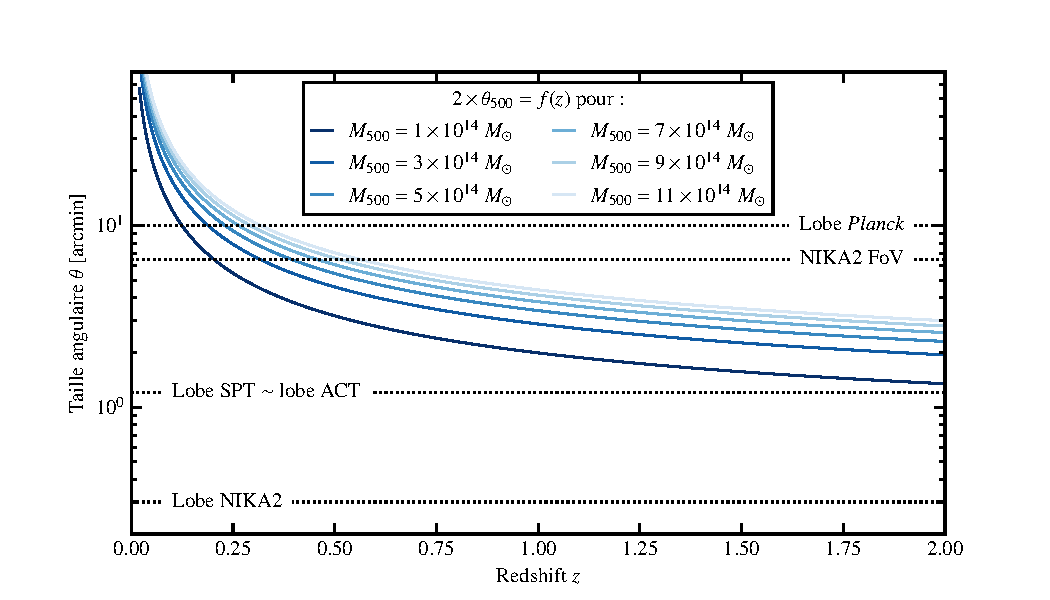
\includegraphics[width=.85\linewidth]{Figures/chap_nk/angular_sizes.pdf}
    \caption{
        Évolution du diamètre angulaire caractéristique $2\theta_{500}$ d'amas de galaxies de différentes masses avec le redshift.
        Les lobes de NIKA2 ($\sim 18$'' à 150 GHz), SPT ($\sim 1.2$'), ACT ($\sim 1.4$'), et \textit{Planck} ($\sim 10$') sont représentés à titre indicatif, de même que le champ de vue instantané (FoV pour \textit{field of view}) de NIKA2 (6.5').
    }
    \label{fig:nk_angular_sizes}
\end{figure*}

La résolution d'amas de galaxies est cruciale pour l'étude de leurs propriétés physiques.
En effet, les observations réalisées par un instrument fournissent une image du ciel convoluée par son lobe.
Par conséquent, la carte d'un amas de galaxies plus petit que la résolution de l'instrument qui l'observe est principalement une carte du lobe de l'instrument, qui ne permet pas une étude détaillée de la structure de l'amas.
C'est pourquoi les cartes de l'effet SZ construites par la collaboration \textit{Planck} \cite{planck_collaboration_planck_2016}, de résolution angulaire $\sim 10$', permettent seulement l'étude détaillée d'amas proches et massifs (comme l'amas de Coma, $z = 0.023, \, M_{500} \simeq 7 \times 10^{14} \;M_\odot$ \cite{ade_planck_2013}).

De la même façon, résoudre un amas (c'est-à-dire l'observer avec un lobe plus petit que son rayon caractéristique) ne permet pas nécessairement un grand niveau de détail dans l'extraction de ses propriétés physiques.
Pour des études précises, il est donc nécessaire que la taille angulaire de l'amas soit non seulement supérieure à la taille du lobe de l'instrument utilisé, mais aussi grande devant celle-ci.
C'est pourquoi les instruments ayant une résolution de l'ordre de la minute d'arc, comme SPT et ACT, ne permettent pas l'étude détaillée d'amas distants: au delà d'un redshift de 0.5, les tailles d'amas $2\theta_{500}$ ne sont au maximum que cinq fois plus grands que les lobes de ces instruments.
La cartographie détaillée de l'effet SZ dans les amas de galaxies nécessite donc l'utilisation d'un instrument à plus haute résolution angulaire.
Comme le montre la figure \ref{fig:nk_angular_sizes}, le lobe de NIKA2 à 150 GHz est inférieur par au moins un ordre de grandeur au diamètre angulaire $2\theta_{500}$ de tous les amas de masse $M_{500} > 3 \times 10^{14} \;M_\odot$, quel que soit leur redshift.
NIKA2 est donc un instrument idéal pour les observations SZ à haute résolution des amas de galaxies distants de l'Univers.

\subsubsection{Grande sensibilité} % -------------------------------------------------- %
La cartographie de l'effet SZ en direction d'amas de galaxies requiert une grande sensibilité.
En effet, la distorsion spectrale due à l'effet SZ est faible.
Dans le cas d'observations avec NIKA2 à 150 GHz, la brillance de surface maximale en direction des amas est de l'ordre du mJy/beam; à titre comparatif, la densité de flux d'Uranus à cette fréquence est de l'ordre de la dizaine de Jy/beam, de même que les fluctuations du bruit de l'atmosphère (ce point sera traité au chapitre suivant).
Par conséquent, une grande sensibilité est nécessaire à la mesure de l'effet SZ dans un temps raisonnable.
NIKA2 est capable de cartographier environ 1400 arcmin$^2$ avec un niveau de bruit de 1 mJy en une heure, ce qui permet d'atteindre le niveau de bruit requis pour la détection de l'effet SZ rapidement, comme discuté dans l'équation (\ref{eq:nk_time}).

\vspace{20pt}

Ainsi, les caractéristiques instrumentales de NIKA2 en font un instrument de choix pour étudier avec un grand niveau de détail les amas de galaxies lointains, non-résolus par \textit{Planck} et difficilement par SPT ou ACT.

% ------------------------------------------------------------------------------------- %
\subsection{Échantillon du grand programme SZ}

Le temps alloué aux observations du LPSZ a été réparti sur un échantillon d'environ cinquante amas de galaxies.
Cet échantillon est l'une des grandes forces du programme: il couvre une grande gamme de masses ($M_{500} \in [3,\,11] \times 10^{14} \;M_\odot$) à haut redshift ($z \in [0.5,\,0.9]$), avec des amas sélectionnés dans des catalogues SZ.
Il est représenté en figure \ref{fig:lpsz_sample}.

Comme nous l'avons discuté au chapitre précédent (voir \ref{sec:sz}), les échantillons sélectionnés par effet SZ ont l'avantage d'être proches d'échantillons sélectionnés en masse.
En effet, le paramètre de Compton intégré étant lié au contenu en énergie thermique de l'amas, il est étroitement lié à la masse (voir section \ref{sec:scaling:sz}, page \pageref{sec:scaling:sz}).
Ainsi, un échantillon construit avec pour critère une valeur de $Y$ supérieure à un seuil choisi sélectionnera les amas sur un critère lié à leur masse, ce qui permet d'éviter de favoriser un type d'amas particulier.
Un tel échantillon est alors dit représentatif, puisque la distribution des propriétés physiques des amas le constituant suit \prior\ la même distribution que les amas de l'Univers dans la gamme de masse considérée.
À titre d'exemple, les amas sélectionnés selon leur pic de luminosité en X ne sont pas représentatifs: la brillance de surface X étant proportionnelle au carré de la densité d'électrons intégrée le long de la ligne de visée (équation \ref{eq:x_brightness}), une telle sélection favorise les amas à cœur dense, qui présentent la caractéristique générale d'être plus relaxés (voir discussion sur les amas à cœur froid en \ref{sec:lpsz_sci}).

La sélection de l'échantillon a donc été basée sur les catalogues SZ existant au début du programme, à savoir les catalogues \textit{Planck} et ACT \cite{planck_collaboration_planck_2016-2, hasselfield_atacama_2013}.
Les amas ont été choisis parmi ceux présents dans les catalogues et visibles depuis le télescope de 30 mètres de l'IRAM (cf. \ref{sec:30m_geo} et figure \ref{fig:30m_sky}), et de manière à couvrir la gamme de masse considérée de manière homogène.
Pour cela, dix \guillemotleft boites \guillemotright\ ont été définies, délimitant deux intervalles en redshift et cinq en masse.
Cinq amas ont été tirés au hasard pour remplir chacune de ces boites, dans le catalogue ACT pour les deux boites de basse masse, et dans le catalogue \textit{Planck} pour les autres.
Dans les deux cas, les estimateurs de masse utilisés pour la répartition sont calculés à partir du signal SZ intégré mesuré par les relevés en utilisant la relation d'échelle de \cite{arnaud_universal_2010}.
Sans cette procédure de division en boîtes du plan masse-redshift, les amas auraient été sélectionnés aléatoirement dans les catalogues \textit{Planck} et ACT, et leur distribution en masse et en redshift aurait suivi la fonction de masse sous-jacente.
À l'inverse, l'échantillon du grand programme SZ constitue une couverture homogène de la gamme de masse et de redshift considérée.
Nous verrons en \mypageref{sec:scaling:intercept_bias} l'impact de cette sélection sur l'ajustement de la relation d'échelle masse-observable à partir des données du grand programme SZ.

\begin{figure*}[t]
    \centering
    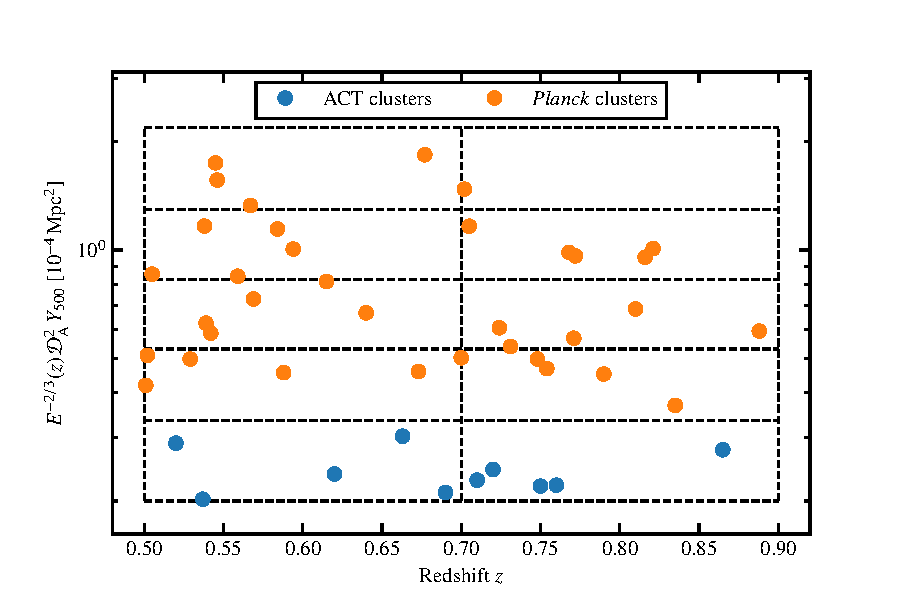
\includegraphics[width=.8\linewidth]{Figures/Chap_nk/lpsz_sample.pdf}
    \caption{
        Distribution des amas du grand programme SZ dans le plan redshift -- paramètre de Compton intégré.
        Les points bleu et orange représentent respectivement les amas extraits des catalogues ACT \cite{hasselfield_atacama_2013} et \textit{Planck} \cite{planck_collaboration_planck_2016-2}.
        Les lignes noires pointillées représentent les limites des boites utilisées pour construire l'échantillon.
    }
    \label{fig:lpsz_sample}
\end{figure*}

Le suivi SZ à haute résolution d'un échantillon d'amas aussi nombreux, à des redshifts supérieurs à 0.5, et sur une si grande gamme de masse est sans précédent.
Il permettra de comparer les propriétés d'amas de galaxies distants, mesurées en SZ avec une grande résolution angulaire, à celles mesurées sur des échantillons d'amas proches, mesurés en X ou en SZ avec une faible résolution.

Comme nous l'avons mentionné, le temps alloué au LPSZ est de 300 heures d'observation.
La distribution de ces heures entre les différents amas de l'échantillon a été calculée de façon à obtenir un signal de qualité équivalente pour chacun des amas.
Le temps alloué à un amas est ainsi calculé comme le temps d'observation nécessaire à l'obtention d'un rapport signal-sur-bruit du profil de brillance de surface SZ de $3\sigma$ au rayon caractéristique $R_{500}$.
Ce calcul est basé sur plusieurs hypothèses.
D'une part, il a été supposé que le profil de pression de chaque amas était donné par le profil de pression universel du milieu intra-amas d'\myciteauthor{arnaud_universal_2010}, discuté en \mypageref{sec:univ_press_prof}.
D'autre part, le calcul a été fait dans l'hypothèse où la masse $M_{500}$ des amas de l'échantillon était égale à celle donnée par les catalogues \textit{Planck} et ACT dans lesquels les amas sont choisis.
Celles-ci ont été obtenues par l'utilisation d'une relation d'échelle liant l'observable des relevés SZ à la masse.
À partir de ces deux hypothèses, un profil de paramètre de Compton a été calculé pour chaque amas.
Le temps d'observation en a été déduit en suivant le calcul présenté en équation (\ref{eq:nk_time}) comme le temps nécessaire pour atteindre un niveau de bruit trois fois inférieur à la valeur de ce profil à $R_{500}$.
On note que tout écart aux hypothèses émises au cours de ce calcul, par exemple sur le profil de pression du milieu intra-amas ou sur la relation d'échelle masse-observable, entraine un changement dans la qualité du signal attendu.
Ainsi, un amas dont la masse est mal estimée par la relation d'échelle, ou dont le profil de pression présente un écart au profil universel, peut présenter une qualité de données significativement différente de celle attendue.
De plus, les temps d'observation ont été calculés avant la construction de NIKA2, et les performances réelles de l'instrument étaient encore inconnues.
Par conséquent, il est possible que la qualité générale des observations NIKA2 des amas de l'échantillon soient moins bonne qu'attendu.
Ce point nécessite une grande précaution, car pour étalonner les outils nécessaires à la cosmologie, l'échantillon doit être représentatif, et les observations des amas doivent avoir une qualité équivalente afin de ne pas donner un poids trop important à un type d'amas donné.

% ------------------------------------------------------------------------------------- %
\subsection{Objectifs scientifiques du grand programme SZ} \label{sec:lpsz_sci}

Le grand programme SZ exploite les performances de NIKA2 et sa capacité à mesurer l'effet SZ à haute résolution dans le but de répondre à plusieurs questions de la cosmologie avec des amas de galaxies.

\subsubsection{Études détaillées des amas de l'échantillon} % -------------------------- %
Comme discuté en section \ref{sec:nk_sz}, les performances et caractéristiques de NIKA2 sont en adéquation avec les besoins pour l'étude à haute résolution d'amas de galaxies.
Par conséquent, les observations des amas du LPSZ avec NIKA2 permettent de les imager avec un grand niveau de détail.
Les études des propriétés individuelles de chaque amas sont alors rendues possibles.

Les résultats de ces études seront rendus disponibles par la collaboration NIKA2 à la fin du programme.
Certaines études individuelles le sont déjà, notamment les deux premières études individuelles du LPSZ: \cite{ruppin_first_2018}, et \cite{keruzore_exploiting_2020}, menée au cours de cette thèse et présentée au chapitre \ref{chap:actj0215}.
Les produits finaux seront pour chacun des amas de l'échantillon du LPSZ:
\begin{itemize}[leftmargin=*]
\setlength\itemsep{5pt}
    \item Les cartes NIKA2 de la région de l'amas, à 150 et 260 GHz, étalonnées et soustraites du bruit corrélé (voir chapitre \ref{chap:decorr});
    \item Le profil de pression de l'amas mesuré avec le logiciel \texttt{PANCO2}, développé dans le cadre de cette thèse, et présenté au chapitre \ref{chap:panco};
    \item Les valeurs des grandeurs caractéristiques intégrées de l'amas, $R_{500}$, $Y_{500}$, et $M_{500}$, qui pourront être utilisées par la communauté pour améliorer la mesure de la relation d'échelle masse-observable dans les analyses cosmologiques de catalogues d'amas de galaxies -- voir section \ref{sec:scaling}, et chapitre \ref{chap:scaling}.
\end{itemize}
Toutes ces informations seront rendues publiques sous la forme d'un catalogue, et utilisables par la communauté pour combiner les informations issues de l'analyse des amas du LPSZ avec d'autres données futures, afin d'enrichir la connaissance de la physique des amas de galaxies grâce à l'échantillon du LPSZ.

\subsubsection{Profil de pression moyen des amas de galaxies} % ----------------------- %
L'un des objectifs principaux du LPSZ est la mesure du profil de pression moyen d'amas de galaxies à haut redshift.
Le profil universel d'\myciteauthor{arnaud_universal_2010}, obtenu par l'exploitation de l'échantillon REXCESS en X à $z < 0.2$, a été utilisé dans la construction de plusieurs catalogues d'amas en SZ, notamment par les collaborations ACT \cite{hilton_atacama_2021} et \textit{Planck} \cite{planck_collaboration_planck_2016-2}.
Il est intéressant de noter que dans les deux cas, les catalogues sont construits à partir de détections des amas par effet SZ, et qu'ils comportent des amas à des redshifts bien plus grands que 0.2, redshift maximal du suivi REXCESS.
Deux questions se posent alors:
\begin{itemize}[leftmargin=*]
\setlength\itemsep{5pt}
\item
    Le profil de pression moyen des amas pourrait-il être différent de la mesure d'\citeauthor{arnaud_universal_2010}? \\
    Une différence pourrait avoir plusieurs origines.
    D'une part, les mesures de profil de pression en X requièrent l'estimation de la température du milieu intra-amas par spectroscopie, qui présente plusieurs incertitudes systématiques complexes \cite{bohringer_x-ray_2010}.
    Il est donc possible que les profils de pression mesurés en X et en SZ ne soient pas strictement équivalents.
    D'autre part, le profil de pression moyen des amas pourrait évoluer avec le redshift.
    Dans ce cas, l'utilisation d'un profil de pression évalué à $z < 0.2$ serait inadaptée à la détection d'amas aussi lointains que $z=2$ (dans le cas du relevé ACT), ou même jusqu'à $z=1$ (dans le cas de \textit{Planck}).
    Enfin, ce profil de pression pourrait ne pas être représentatif de tous les amas de l'Univers, à cause des effets de sélection caractéristiques des échantillons d'amas détectés en X discutés précédemment.
\item
Quel impact aurait une variation du profil de pression moyen sur les analyses cosmologiques basées sur l'effet SZ? \\
    Comme nous l'avons vu, la connaissance du profil de pression moyen des amas est nécessaire à l'extraction de catalogues d'amas à partir d'observations millimétriques.
    Une variation du profil -- avec la méthode de détection ou avec le redshift -- pourrait ainsi \prior\ modifier les catalogues issus des cartes de \textit{Planck} et ACT, et donc les résultats des mesures de paramètres cosmologiques.
    Cet impact a été quantifié dans le cas d'analyses du spectre de puissance de l'effet SZ par \myciteauthor{ruppin_impact_2019}, en analysant la carte de paramètre de Compton issue des données de \textit{Planck} \cite{planck_collaboration_planck_2016} avec différents profils de pression moyens.
    Leurs résultats montrent qu'une modification de l'amplitude du profil de pression aussi faible que 15\% peut affecter significativement les résultats des analyses cosmologiques.
\end{itemize}

L'objectif du LPSZ est de répondre à ces questions en mesurant le profil de pression moyen des amas de son échantillon.
Plusieurs études récentes s'intéressent à de possibles variations du profil de pression moyen des amas avec le redshift, mais utilisent principalement des observations X (\eg\ \cite{mcdonald_redshift_2014, ghirardini_evolution_2021}).
L'utilisation de données SZ à haute résolution offrira des contraintes complémentaires, et créera l'opportunité de comparaisons de résultats multilongueur d'onde.

\subsubsection{Combinaisons multilongueur d'onde et propriétés thermodynamiques} % -- %
Comme nous l'avons vu au chapitre précédent, les observations de l'effet tSZ permettent de sonder la pression thermique des électrons du milieu intra-amas.
Si celle-ci donne des informations importantes sur les amas, d'autres propriétés thermodynamiques revêtent également une grande importance pour l'étude de la physique de ces objets, et ne sont pas mesurables par l'effet tSZ seul.

C'est la raison pour laquelle le LPSZ comporte un suivi de tous ses amas à d'autres longueurs d'onde, complémentaires à l'effet SZ.
Un suivi en X avec les satellites \textit{XMM-Newton} et \textit{Chandra} est notamment l'un des grands points forts du programme.
La combinaison de ces observations avec celles effectuées avec NIKA2 permettra la première étude des propriétés thermodynamiques d'un échantillon d'amas à $z > 0.5$ avec des données X et SZ de qualité comparable.
En effet, comme détaillé en section \mypageref{sec:cluster_obs}, les observations X et SZ sont très complémentaires, puisqu'elles sondent respectivement la densité et la pression du milieu intra-amas qui peuvent être combinées pour calculer la masse de l'amas.
Mais d'autres propriétés peuvent également être calculées par cette combinaison.
Par exemple, le profil de température du milieu intra-amas, dans l'hypothèse d'un gaz parfait, s'écrit:
\begin{equation}
    \label{eq:temperature}
    k_\textsc{b}T_\e(r) = P_\e(r) / n_\e(r),
\end{equation}
et permet d'étudier l'état dynamique de l'amas, pouvant révéler des mécanismes de fusion de plusieurs sous-amas (\eg\ \cite{adam_mapping_2017,ruppin_unveiling_2020}).
Les mesures de température permettent également l'étude des corrections relativistes à l'effet SZ, qui dépendent de cette dernière, comme décrit en section \mypageref{sec:sz}.
On peut également définir le paramètre d'entropie, introduit par \myciteauthor{voit_modified_2002} comme:
\begin{equation}
    \label{eq:entropy}
    K_\e(r) = P_\e(r) \, n_\e(r)^{-5/3}.
\end{equation}
Cette quantité, souvent nommée entropie du milieu intra-amas, est liée au caractère adiabatique de l'évolution de l'amas; dans l'hypothèse où le milieu intra-amas est un gaz parfait monoatomique d'électrons, on peut écrire la loi de Laplace $PV^\gamma = {\rm cste}$ comme:
\begin{equation}
    P_\e \, n_\e^{-5/3} = {\rm cste},
\end{equation}
et la combinaison avec l'équation (\ref{eq:entropy}) permet d'identifier $K_\e$ comme le terme constant.
Ce paramètre d'entropie est donc intimement lié à l'entropie thermodynamique du milieu intra-amas: la formule de de Sackur-Tetrode donne l'entropie par particule d'un gaz parfait $s$, qui peut s'exprimer en fonction de $K_\e$ comme:
\begin{equation}
    \label{eq:entropy_s_K}
    s = k_\textsc{b} \ln K_\e^{3/2} + {\rm cste}.
\end{equation}
Le paramètre $K_\e$ peut donc être interprété comme une mesure en échelle exponentielle de l'entropie par particule $s$, ou encore comme une mesure du nombre d'états microscopiques $\Omega$ par comparaison de l'équation (\ref{eq:entropy_s_K}) et de l'équation de Boltzmann, $S = k_\textsc{b} \ln \Omega$.

Le paramètre d'entropie, simplement nommé entropie dans la suite, est d'un intérêt considérable pour l'étude de la physique des amas (voir \cite{voit_tracing_2005} -- en particulier la section IV -- pour une revue).
Il a historiquement été étudié dans des simulations d'amas de galaxies.
Dans le cas où seuls les processus gravitationnels sont considérés pour la formation des amas, l'entropie dans les amas croît en loi de puissance avec le rayon.
Ce comportement est observé dans les simulations à $N$ corps considérant des particules de matière sombre seulement, donnant des profils d'entropie de forme $K_\e(r) \propto r^{1.1}$ \cite{voit_tracing_2005}.
Dans les simulations plus complexes, de même que dans les amas réels, on observe un écart à ce comportement, en particulier dans le cœur des amas.
Cet écart est dû aux phénomènes tels que des fusions de sous-structures, ou encore l'injection d'énergie par des noyaux actifs de galaxies ou des explosions de supernovas, principalement localisés dans le cœur des amas, et qui augmentent l'entropie du gaz.
Il est illustré en figure \ref{fig:entropy_rexcess} pour l'échantillon REXCESS, discuté précédemment.
On voit que le profil d'entropie des amas suit bien $K_\e(r) \propto r^{1.1}$ à grand rayon, mais que le centre des profils montre un écart significatif.
Cet écart est d'autant plus fort que le cœur des amas est perturbé: les profils bleus, correspondant aux amas \textit{cool-core}, sont plus en accord avec $K_\e(r) \propto r^{1.1}$ que les courbes rouges, correspondant aux amas perturbés.
L'entropie $K_\e$ représente donc un traceur de l'histoire thermique du milieu intra-amas, son écart au profil d'entropie purement gravitationnel donnant une forme de mémoire des processus non-gravitationnels ayant eu lieu au sein des amas.

\begin{figure*}[t]
    \centering
    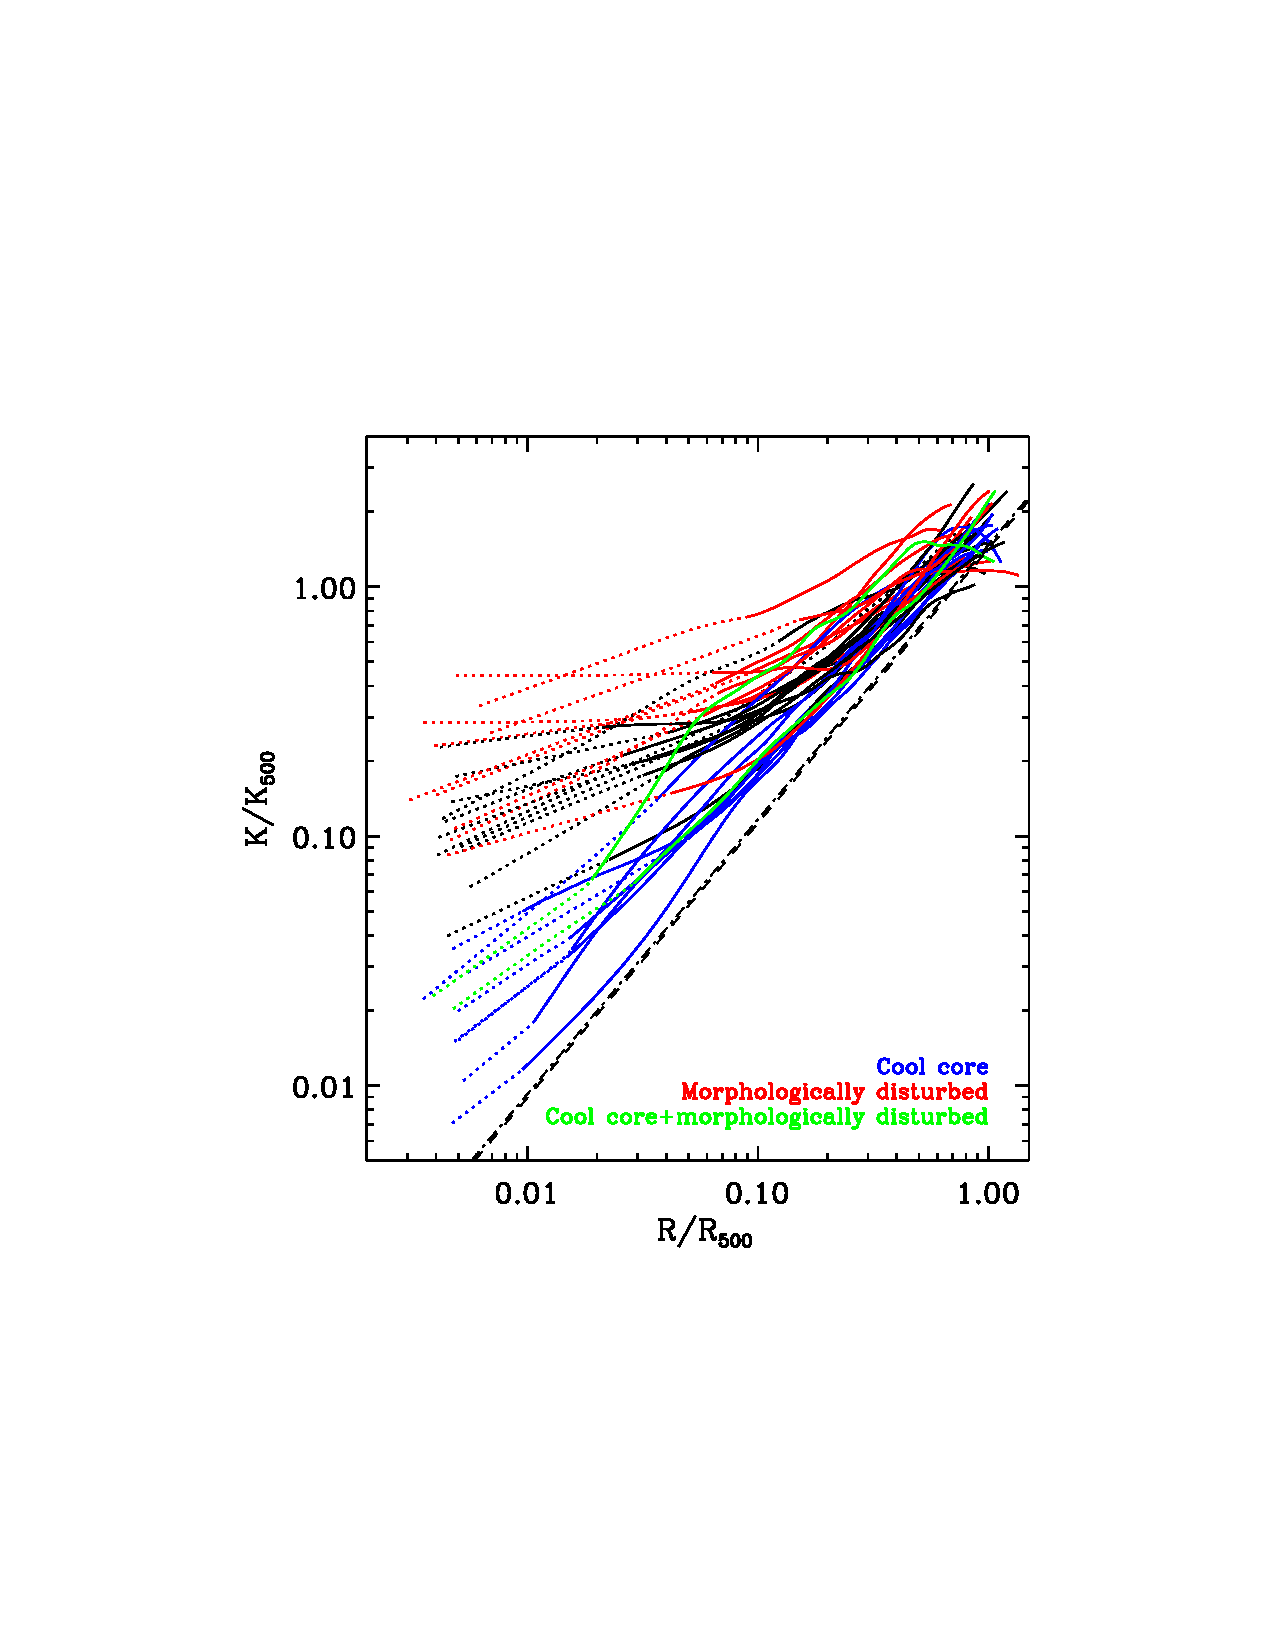
\includegraphics[width=.6\linewidth]{Figures/Chap_nk/entropy_pratt.pdf}
    \caption{
        Profils d'entropie mesurés à partir des observations \textit{XMM-Newton} des amas de l'échantillon REXCESS.
        Les lignes pointillées noires marquent le profil en $r^{1.1}$ attendu pour une formation d'amas purement par effondrement gravitationnel.
        Les courbes bleues et rouges sont respectivement les profils d'amas classifiés comme \textit{cool-core} et à cœur perturbé.
        Figure extraite de \cite{pratt_gas_2010}.
    }
    \label{fig:entropy_rexcess}
\end{figure*}

Les combinaisons de mesures X et SZ permettront donc au LPSZ d'étudier en détail les propriétés thermodynamiques du milieu intra-amas jusqu'à un redshift de $0.9$, pour un échantillon d'amas sélectionnés en SZ.
Outre leur importance directe pour la physique des amas, ces mesures pourront être utilisées pour classer les amas en fonction de leurs propriétés dynamiques.
En particulier, on trouve dans l'Univers des amas à cœur froid (ou \textit{cool core}), dont les propriétés centrales indique un état de relaxation, et les amas au cœur perturbé.
Ces deux types d'amas ont des propriétés globalement différentes, comme décrit par exemple dans l'étude de \myciteauthor{hudson_what_2010}, qui étudie les différences entre les amas \textit{cool-core} et perturbés sur le critère de 16 propriétés physiques différentes.
En outre, les amas à cœur froid possèdent une entropie centrale bien plus faible que les amas perturbés, caractéristique d'injections d'énergie non-thermiques moins importantes.
Ils ont également une densité centrale plus élevée (et sont ainsi plus facilement détectés en X), ainsi qu'un profil de pression bien plus piqué en leur centre.
Nous avons discuté de l'importance de la mesure du profil de pression moyen des amas de galaxies pour les études cosmologiques; une différence significative entre deux populations d'amas pourrait également avoir un impact sur de telles études.
Les observations du LPSZ, en étudiant la température, l'entropie, et la pression du milieu intra-amas à l'aide d'observations résolues en X et en SZ, pourront distinguer ces populations, et les étudier séparément pour approfondir la connaissance de leurs propriétés thermodynamiques et de leur distribution dans les différentes populations.

De plus, comme nous l'avons discuté au chapitre précédent, les observations SZ permettent de réduire le temps nécessaire par rapport aux observations X permettant les mesures spectroscopiques.
Traditionnellement, les études résolues d'amas faisaient appel à des observations X profondes, afin de pouvoir extraire un profil de température par spectroscopie, et ainsi de pouvoir déduire une mesure du profil de pression.
Avec un profil de pression fourni par les mesures en SZ, la spectroscopie X n'est plus nécessaire pour remonter à la masse.
Toutefois, certains des amas du LPSZ ont été suivis en X avec des observations profondes, permettant les études spectroscopiques.
Pour de telles observations, la combinaison des observations SZ et X (sans spectroscopie) pourra être comparée aux mesures X seules, pour étudier de potentielles différences pouvant être dues aux incertitudes systématiques affectant les mesures de température en spectroscopie X (voir \cite{bohringer_x-ray_2010} pour une revue).

Enfin, des suivis en optique sont également en cours pour les amas du LPSZ, avec le Gran Telescopio Canarias à l'observatoire des Canaries.
Ce suivi spectroscopique permettra d'étudier la distribution des galaxies des amas du LPSZ, ainsi que leurs masses par dispersion des vitesses (voir par exemple \cite{barrena_optical_2020} pour une étude similaire de suivi des amas \textit{Planck} avec le Gran Telescopio Canarias).
De plus, certains des amas du LPSZ font partie d'échantillons d'amas suivis par d'autres instruments; par exemple, l'échantillon CLASH \cite{postman_cluster_2012}, ayant réalisé un suivi d'amas avec le \textit{Hubble Space Telescope} dont les données sont aujourd'hui publiques.
Ces données permettront des études de la masse d'amas du LPSZ par des mesures optiques, en utilisant la dispersion des vitesses pour le suivi spectroscopique et le lentillage gravitationnel pour les données de HST.
Ces estimateurs de masses, comme nous l'avons discuté en \mypageref{sec:cluster_obs}, ne sont pas affectés par le biais hydrostatique, mais peuvent souffrir de biais différents \cite{becker_accuracy_2011, grandis_calibration_2021}.
La comparaison des mesures de masse dans ces suivis avec celles obtenues par combinaison des observations SZ avec NIKA2 et X permettra donc d'étudier ce biais pour une partie de l'échantillon \cite{munoz_echevarria_lpsz-clash_2021}.

\subsubsection{La relation d'échelle} % ----------------------------------------------- %
Comme nous l'avons vu en \ref{sec:scaling}, la connaissance du lien entre la masse d'un amas et son observable dans un relevé est cruciale pour l'exploitation cosmologique du relevé en question.
Tout comme pour le profil de pression moyen du milieu intra-amas, l'étude de ce lien a aujourd'hui principalement été menée en utilisant des amas proches, et des masses souvent mesurées à l'aide uniquement d'observations X (\eg\ \cite{arnaud_universal_2010,planck_collaboration_planck_2011}).
Les mêmes questions se posent alors, interrogeant sur de possibles variations de la relation avec le redshift, avec l'utilisation de données SZ, et sur l'impact de telles variations sur les résultats cosmologiques.

Afin de pouvoir utiliser l'échantillon du LPSZ pour étudier de possibles évolutions de la relation d'échelle, il est nécessaire de connaître la masse des amas.
Comme nous l'avons vu en \ref{sec:sz}, l'effet SZ seul ne permet pas de mesurer la masse d'un amas.
Celle-ci peut cependant être estimée à partir de la combinaison d'observations SZ et X, comme discuté en \ref{sec:x}.
La mesure de la relation d'échelle fera donc appel à la combinaisons des observations SZ et X des amas de l'échantillon détaillée précédemment.
En plus des mesures de masse, l'étude des propriétés thermodynamiques des amas et leur classification basée sur ces propriétés permettra des études systématiques détaillées sur l'impact des propriétés des amas sur la relation d'échelle.
Par exemple, les amas perturbés pourraient suivre une relation d'échelle différente de celle suivie par les amas à cœur froid.
Une étude intéressante serait la réduction de la dispersion autour de la relation d'échelle grâce aux propriétés thermodynamiques des amas, mesurées en détail à l'aide de la combinaison des observations avec NIKA2 et \textit{XMM-Newton} ou \textit{Chandra}.
Jusqu'à présent, les relations d'échelles sont mesurées en supposant des relations en loi de puissance avec une dispersion intrinsèque, comme décrit en section \mypageref{sec:scaling} et au chapitre \ref{chap:scaling}.
Une autre approche pourrait être la réduction de cette dispersion basée sur des propriétés observables des amas.
De telles études sont menées pour mesurer les paramètres cosmologiques à l'aide des supernovas de type Ia, par exemple avec le modèle SALT2 (\cite{guy_salt2_2007}).
Dans de tels travaux (\eg\ \cite{betoule_improved_2014}), le module de distances de chacune des supernovas est corrigé à partir de propriétés observables de l'objet, permettant de réduire la dispersion autour du diagramme de Hubble.
On parle alors des supernovas comme de chandelles standardisables, dont l'exploitation cosmologique repose sur une correction empirique basée sur la mesure des propriétés de chacun des objets.
Des études similaires pourraient être réalisées avec les amas du grand programme SZ, grâce à des observables des amas telles que leurs propriétés thermodynamiques, pour une approche différente à la mesure de relations d'échelle.

Comme nous l'avons mentionné au chapitre précédent, la mesure de relations d'échelle fait intervenir beaucoup d'effets systématiques, tels que les effets de sélection dus au choix des amas de l'échantillon.
Ces effets peuvent être pris en compte au prix d'une modélisation statistique complexe.
L'étude de la relation d'échelle liant la masse au paramètre de Compton intégré au chapitre \ref{chap:scaling}, en utilisant des simulations pour évaluer les différents effets systématiques affectant la mesure de cette relation dans le cadre du LPSZ.

% ===================================================================================== %
\section{La base de données du grand programme SZ de NIKA2}
\label{sec:nk_ami}

% ------------------------------------------------------------------------------------- %
\subsection{Contexte}

Avec l'avancement du grand programme SZ de NIKA2, la quantité d'informations pertinentes pour le programme a augmenté rapidement.
Il a donc été nécessaire de mettre en place un moyen permettant de centraliser ces informations, comportant des renseignements sur les observations NIKA2 ou sur l'existence de données externes.
Un exemple est le besoin d'avoir accès aux coordonnées les plus récentes d'un amas.
En effet, les amas du grand programme SZ sont en majorité issus du catalogue \textit{Planck} \cite{planck_collaboration_planck_2016-2}, construit à partir d'observations dont la résolution est proche de la taille du champ de vue de NIKA2.
Les coordonnées des amas dans ce catalogue sont donc imprécises; en observant à ces coordonnées avec NIKA2, il est possible d'observer à côté de l'amas.
Il est donc préférable d'utiliser les coordonnées d'amas obtenues avec des suivis à plus haute résolution, par exemple en X.
Il est donc important de pouvoir accéder aux coordonnées d'un amas les plus précises possibles.
Un autre exemple d'utilisation est la possibilité d'avoir un outil permettant de connaître rapidement le nombre de \textit{scans} ayant été effectués sur chaque amas, qui peut grandement faciliter la prise de décision sur la liste de sources choisies pour être observées au télescope.
De même, savoir si la collaboration dispose de données X ou optiques associées à un amas permet de choisir les sources considérées pour une analyse multilongueur d'onde.
Enfin, en sauvegardant les résultats des analyses de manière centralisée et accessible, la collaboration pourrait plus facilement garder une traçabilité de l'évolution des résultats avec les développements de logiciels de traitement des données, et choisir des amas de caractéristiques similaires pour une étude d'échantillon.

Il a donc été décidé de construire une base de données du grand programme SZ.
Dans ce contexte, nous avons choisi de collaborer avec les développeurs de AMI (\textit{Atlas Metadata Interface}, \cite{albrand_atlas_2010}), membres du service informatique du Laboratoire de Physique Subatomique et de Cosmologie.
AMI propose un cadre permettant de développer une base de métadonnées, c'est-à-dire un regroupement d'informations sous forme de texte (les données de NIKA2 ou d'autres instruments ne sont pas centralisées).
J'ai été nommé responsable scientifique de cette base de données, et ai pu collaborer avec les développeurs pour établir un cahier des charges, visant à concilier les besoins scientifiques et les possibilités offertes par AMI.

% ------------------------------------------------------------------------------------- %
\subsection{Contenu et interface de la base de données}

Le cahier des charges défini pour la base de données comprend plusieurs exigences.
D'une part, sa structure doit être assez souple pour stocker de l'information évoluant avec le temps, comme les coordonnées les plus précises existant pour chaque amas, l'existence de données externes, etc.
D'autre part, la base de données doit pouvoir être utilisée à plusieurs étapes de la chaîne d'analyse du grand programme SZ:
\begin{itemize}[leftmargin=*]
\setlength\itemsep{0pt}
\item Pendant les observations au télescope, pour accéder aux coordonnées des amas, au temps d'observation nécessaire et déjà effectué, etc.
\item Pendant l'analyse des données brutes, pour accéder à la liste des \textit{scans} associés à un amas et à leurs propriétés.
\item Pendant l'analyse des propriétés physiques des amas, pour accéder aux produits de l'analyse des données brutes (cartes SZ, etc.), aux propriétés des amas (redshift, masse estimée par \textit{Planck}).
\end{itemize}
Chacune des étapes est associée à des besoins d'interactivité différents: une table avec interface graphique est utile pendant les observations et pour avoir des informations rapides sur les amas, mais un accès par ligne de commande peut être plus utile pour l'interface avec les logiciels d'analyse.

La base de données AMI-LPSZ est accessible sur demande pour les membres de la collaboration NIKA2\footnote{\url{https://ami-nika2-lpsz.in2p3.fr/}}.
Elle est composée de plusieurs tables, correspondant chacune à un type de données, et interconnectées.
Les principales sont les suivantes:
\begin{itemize}[leftmargin=*]
\setlength\itemsep{0pt}
\item Une table \texttt{CLUSTER}, dont chaque élément est un amas.
    Les données stockées incluent le nom de chaque amas, ses coordonnées mesurées à partir de différents jeux de données (SZ, optique, X), sa masse et son redshift, le nombre de \textit{scans} à réaliser pour compléter les observations de l'amas, etc.
    Un champ est également présent pour stocker l'information sur l'existence de données externes, par exemple X avec \textit{Chandra} ou \textit{XMM-Newton}, ou submillimétrique pour la contamination par des sources ponctuelles (voir section \ref{sec:decor:pstools}).
\item une table \texttt{SCAN} qui regroupe chaque \textit{scan} effectué par la caméra NIKA2 depuis sa mise en service.
    Les informations associées à chaque \textit{scan} incluent la date et l'heure de l'observation, le nom de la source, le type de \textit{scan}, l'opacité atmosphérique et l'élévation, ou encore les commentaires laissés par les observateurs au moment de sa réalisation.
    J'ai été en charge de l'écriture du programme pour interroger la base de données de l'IRAM dans laquelle ces informations sont consignées pour pouvoir les inclure dans AMI.
    Pour les \textit{scans} dont le nom de source est l'un des amas de galaxies du grand programme SZ, un lien est créé entre le \textit{scan} et l'entrée correspondant à l'amas dans la table \texttt{CLUSTER}, de sorte à ce qu'il soit possible d'extraire la liste des \textit{scans} effectués pour chaque amas.
\item Une table \texttt{CAMPAIGN}, dont chaque élément est une campagne d'observation avec NIKA2.
    Chaque élément de la table \texttt{SCAN} est ainsi associé à une campagne d'observations.
    Cela permet de conserver des informations sur chaque campagne d'observations, comme une météo particulièrement capricieuse ou un problème dans l'acquisition des données, afin de pouvoir éventuellement exclure des \textit{scans} lors des analyses.
\item Une table \texttt{ANALYSIS}, qui répertorie les résultats d'analyse des amas individuels.
    La structure de cette table et son contenus sont toujours en cours de discussion.
    À terme, le but est de garder une trace des analyses des données brutes de NIKA2 (chapitre \ref{chap:decorr}) et des propriétés thermodynamiques (chapitre \ref{chap:panco}) dans AMI.
\end{itemize}

La base de données est accessible de deux façons.
D'une part, l'interface web offre une interface graphique qui permet de chercher des entrées dans les différentes tables.
Ces recherches peuvent être faites sur n'importe quel critère pouvant être construit à partir des différents champs présents dans les tables.
Deux exemples sont présentés en figure \ref{fig:ami_request}: une recherche des amas du programme dans l'intervalle de redshift $0.5 < z < 0.7$, et des \textit{scans} de l'amas \act\ effectués dans des conditions atmosphériques $0.1 < \tau_{225} < 0.2$.
Dans les deux cas, AMI permet d'extraire la liste des objets -- amas dans le premier cas, et \textit{scans} dans le second -- satisfaisant ces conditions, et leurs propriétés.
Chaque élément de la liste peut également être inspecté individuellement.

\begin{figure*}[t]
    \centering
    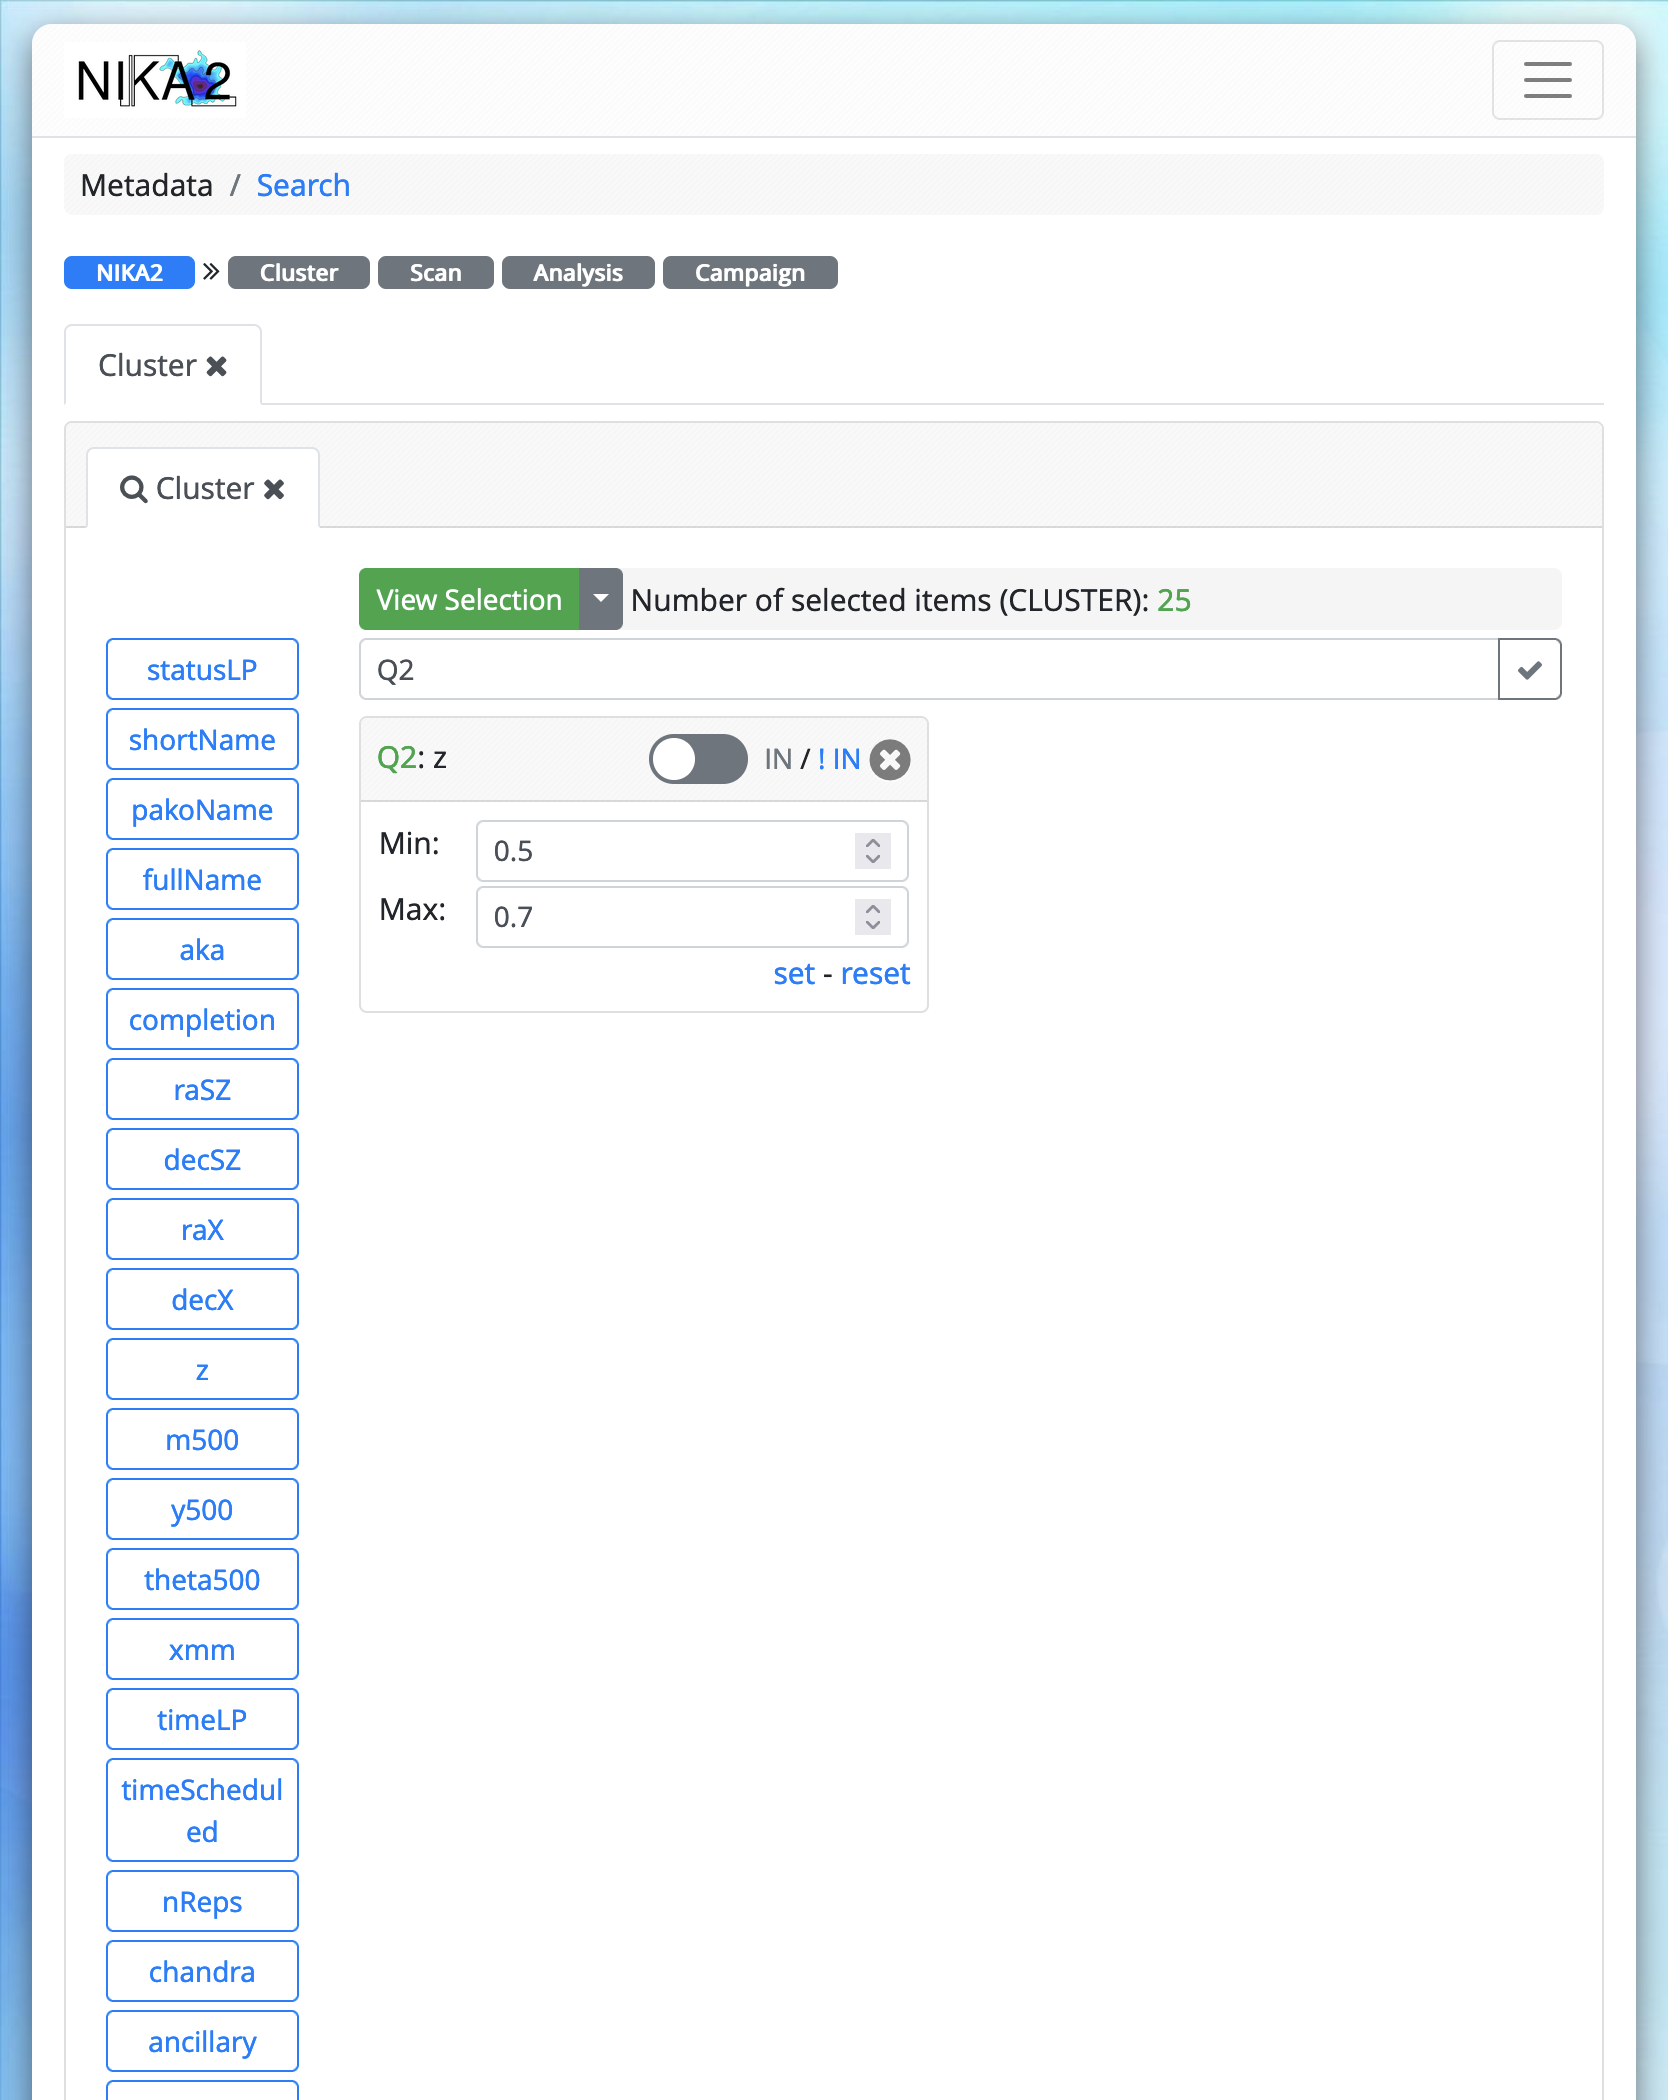
\includegraphics[width=.49\linewidth, trim={0 12cm 0 0}, clip]{Figures/Chap_nk/ami_query_1.png} \hfill
    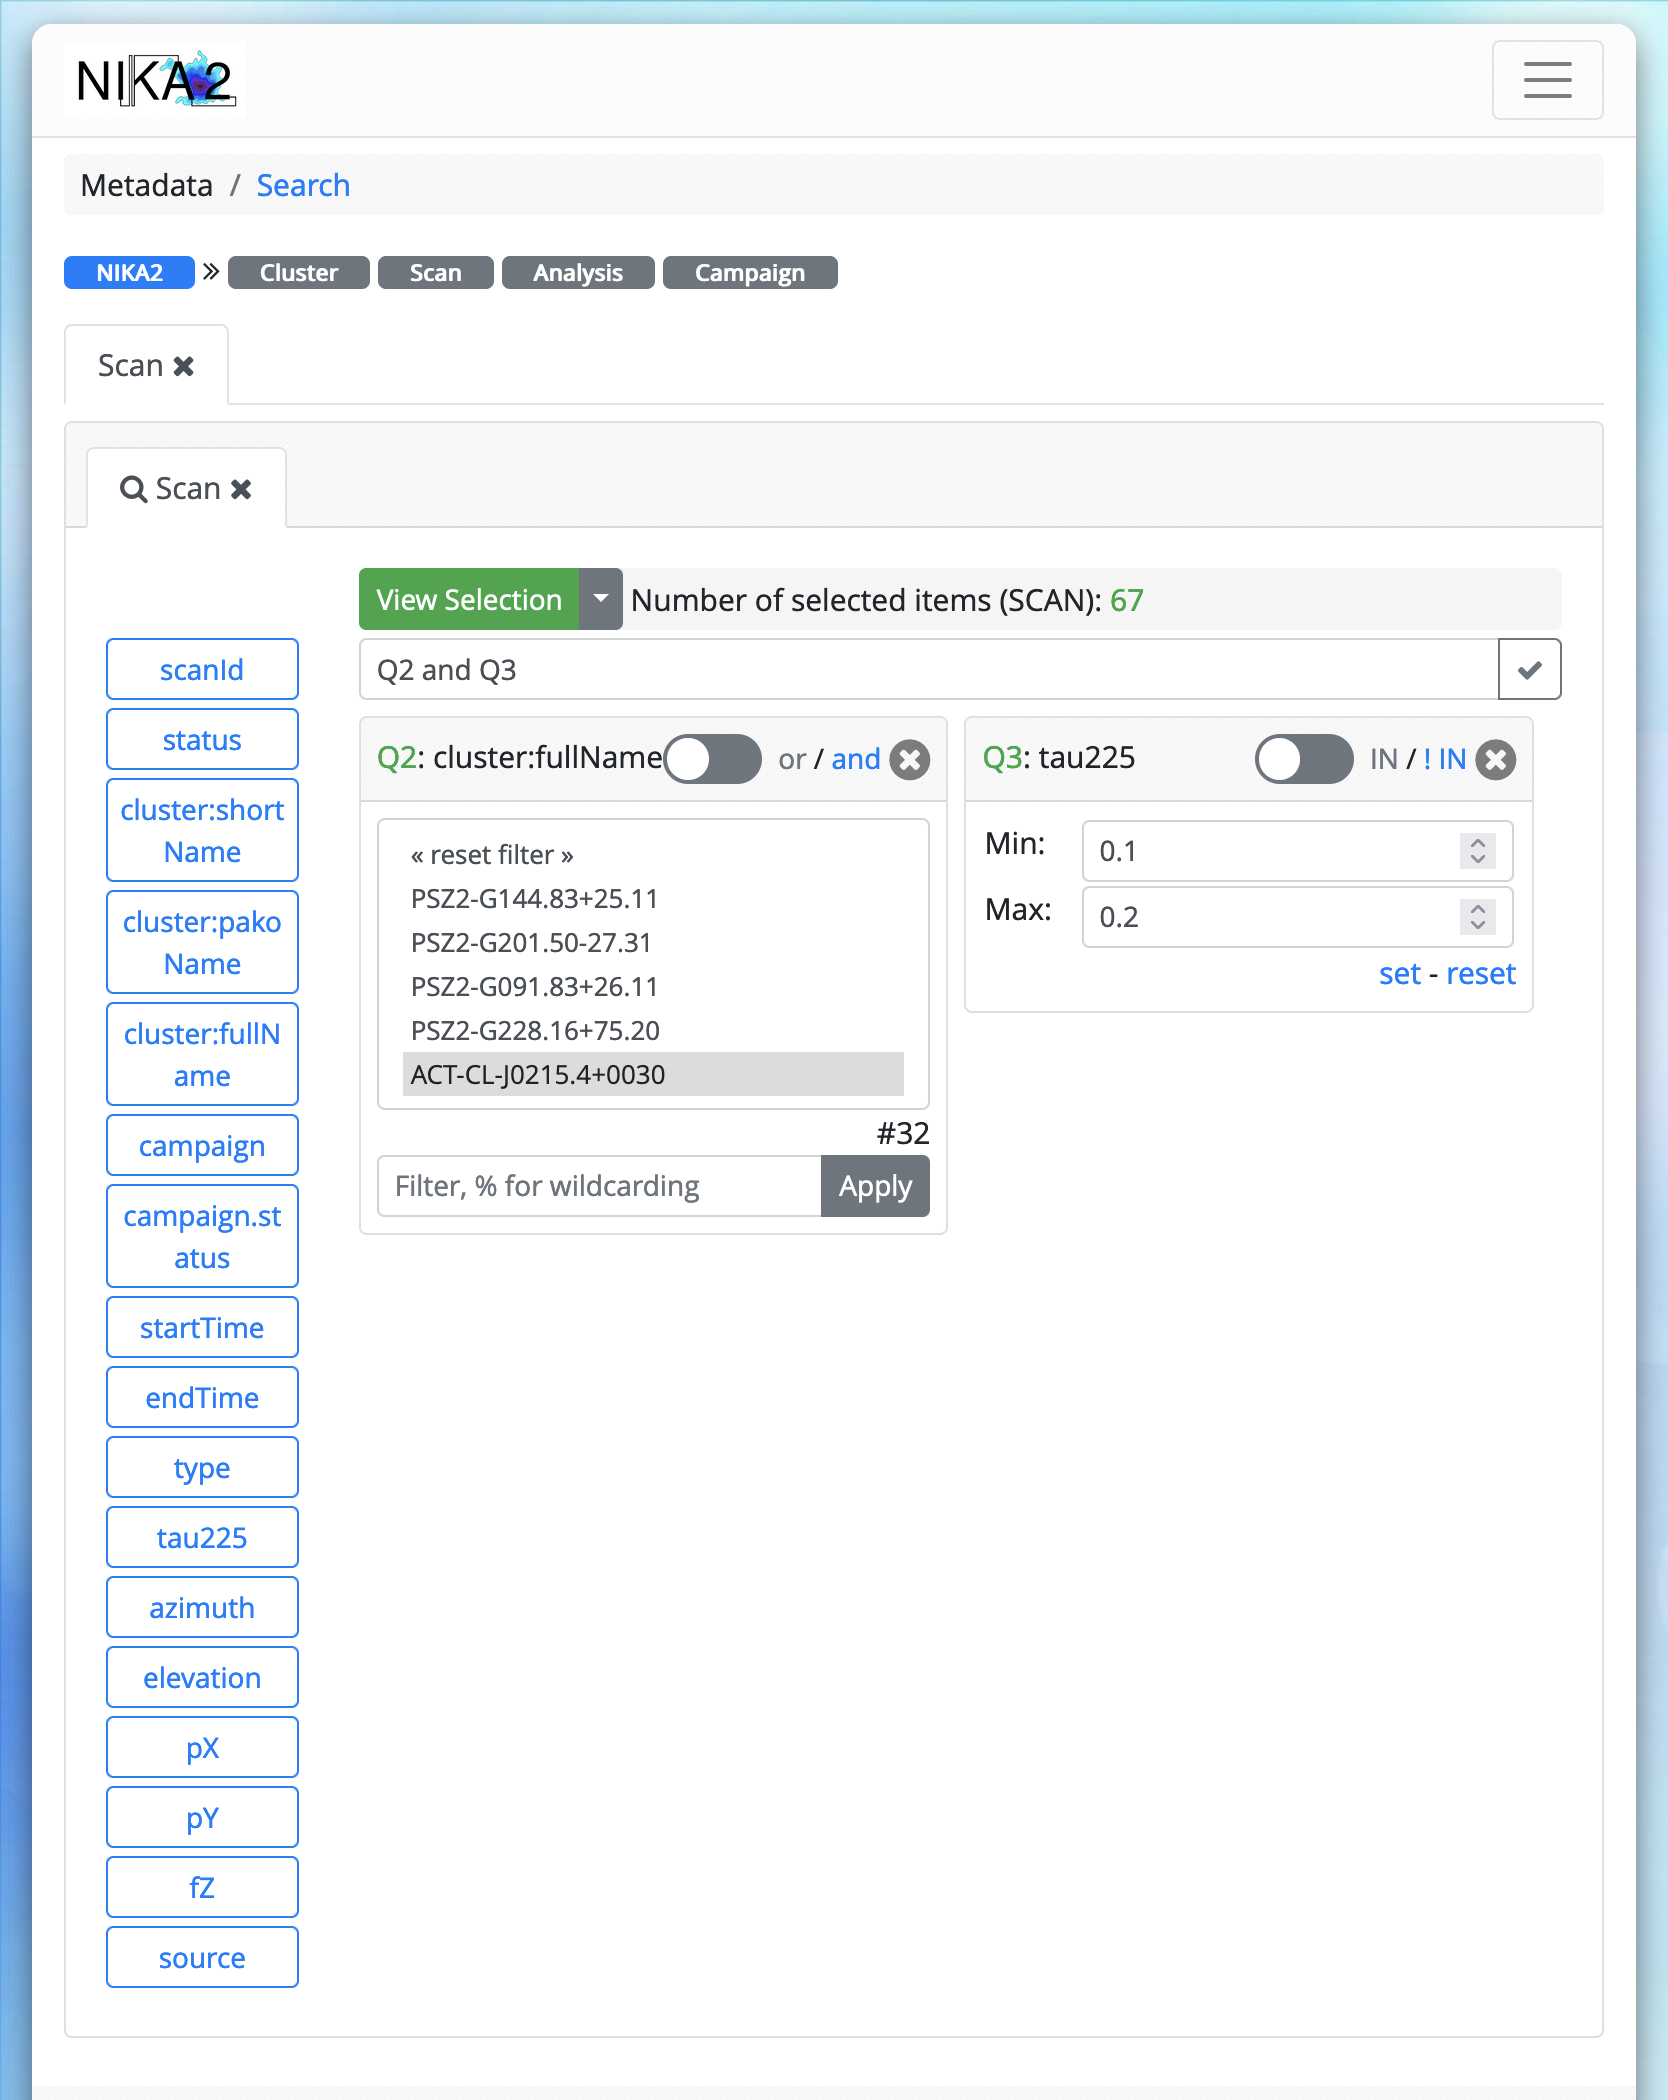
\includegraphics[width=.49\linewidth, trim={0 12cm 0 0}, clip]{Figures/Chap_nk/ami_query_2.png}
    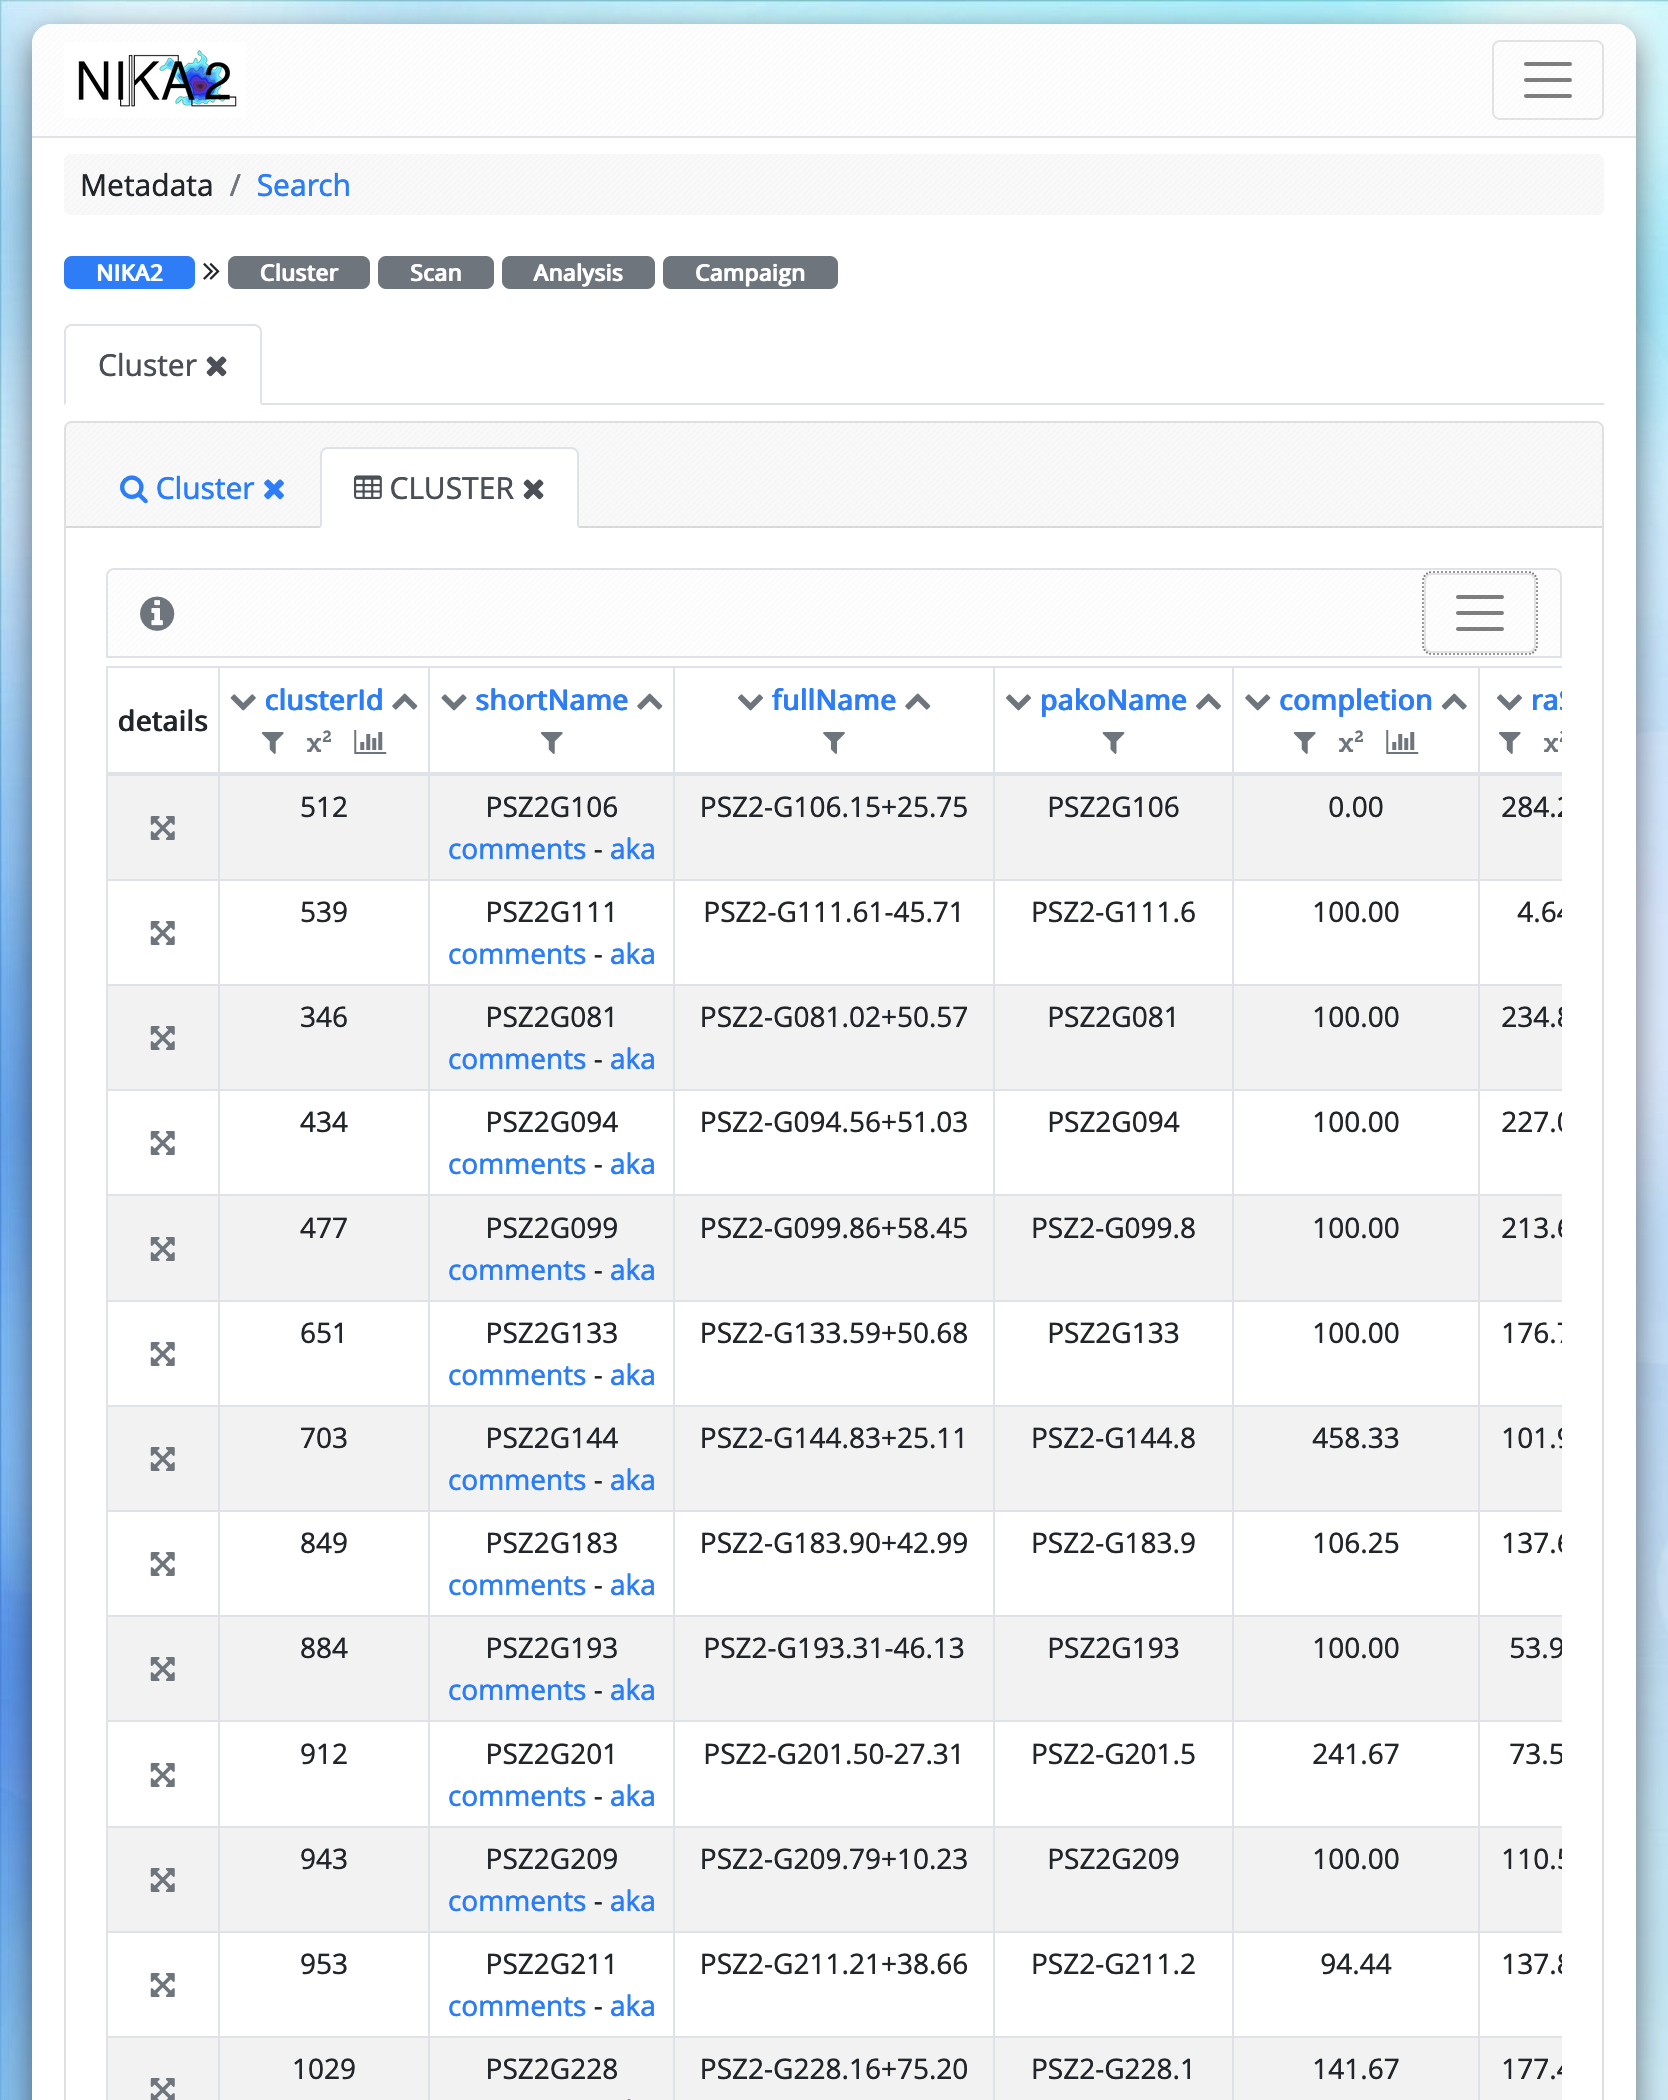
\includegraphics[width=.49\linewidth, trim={0 12cm 0 0}, clip]{Figures/Chap_nk/ami_results_1.png} \hfill
    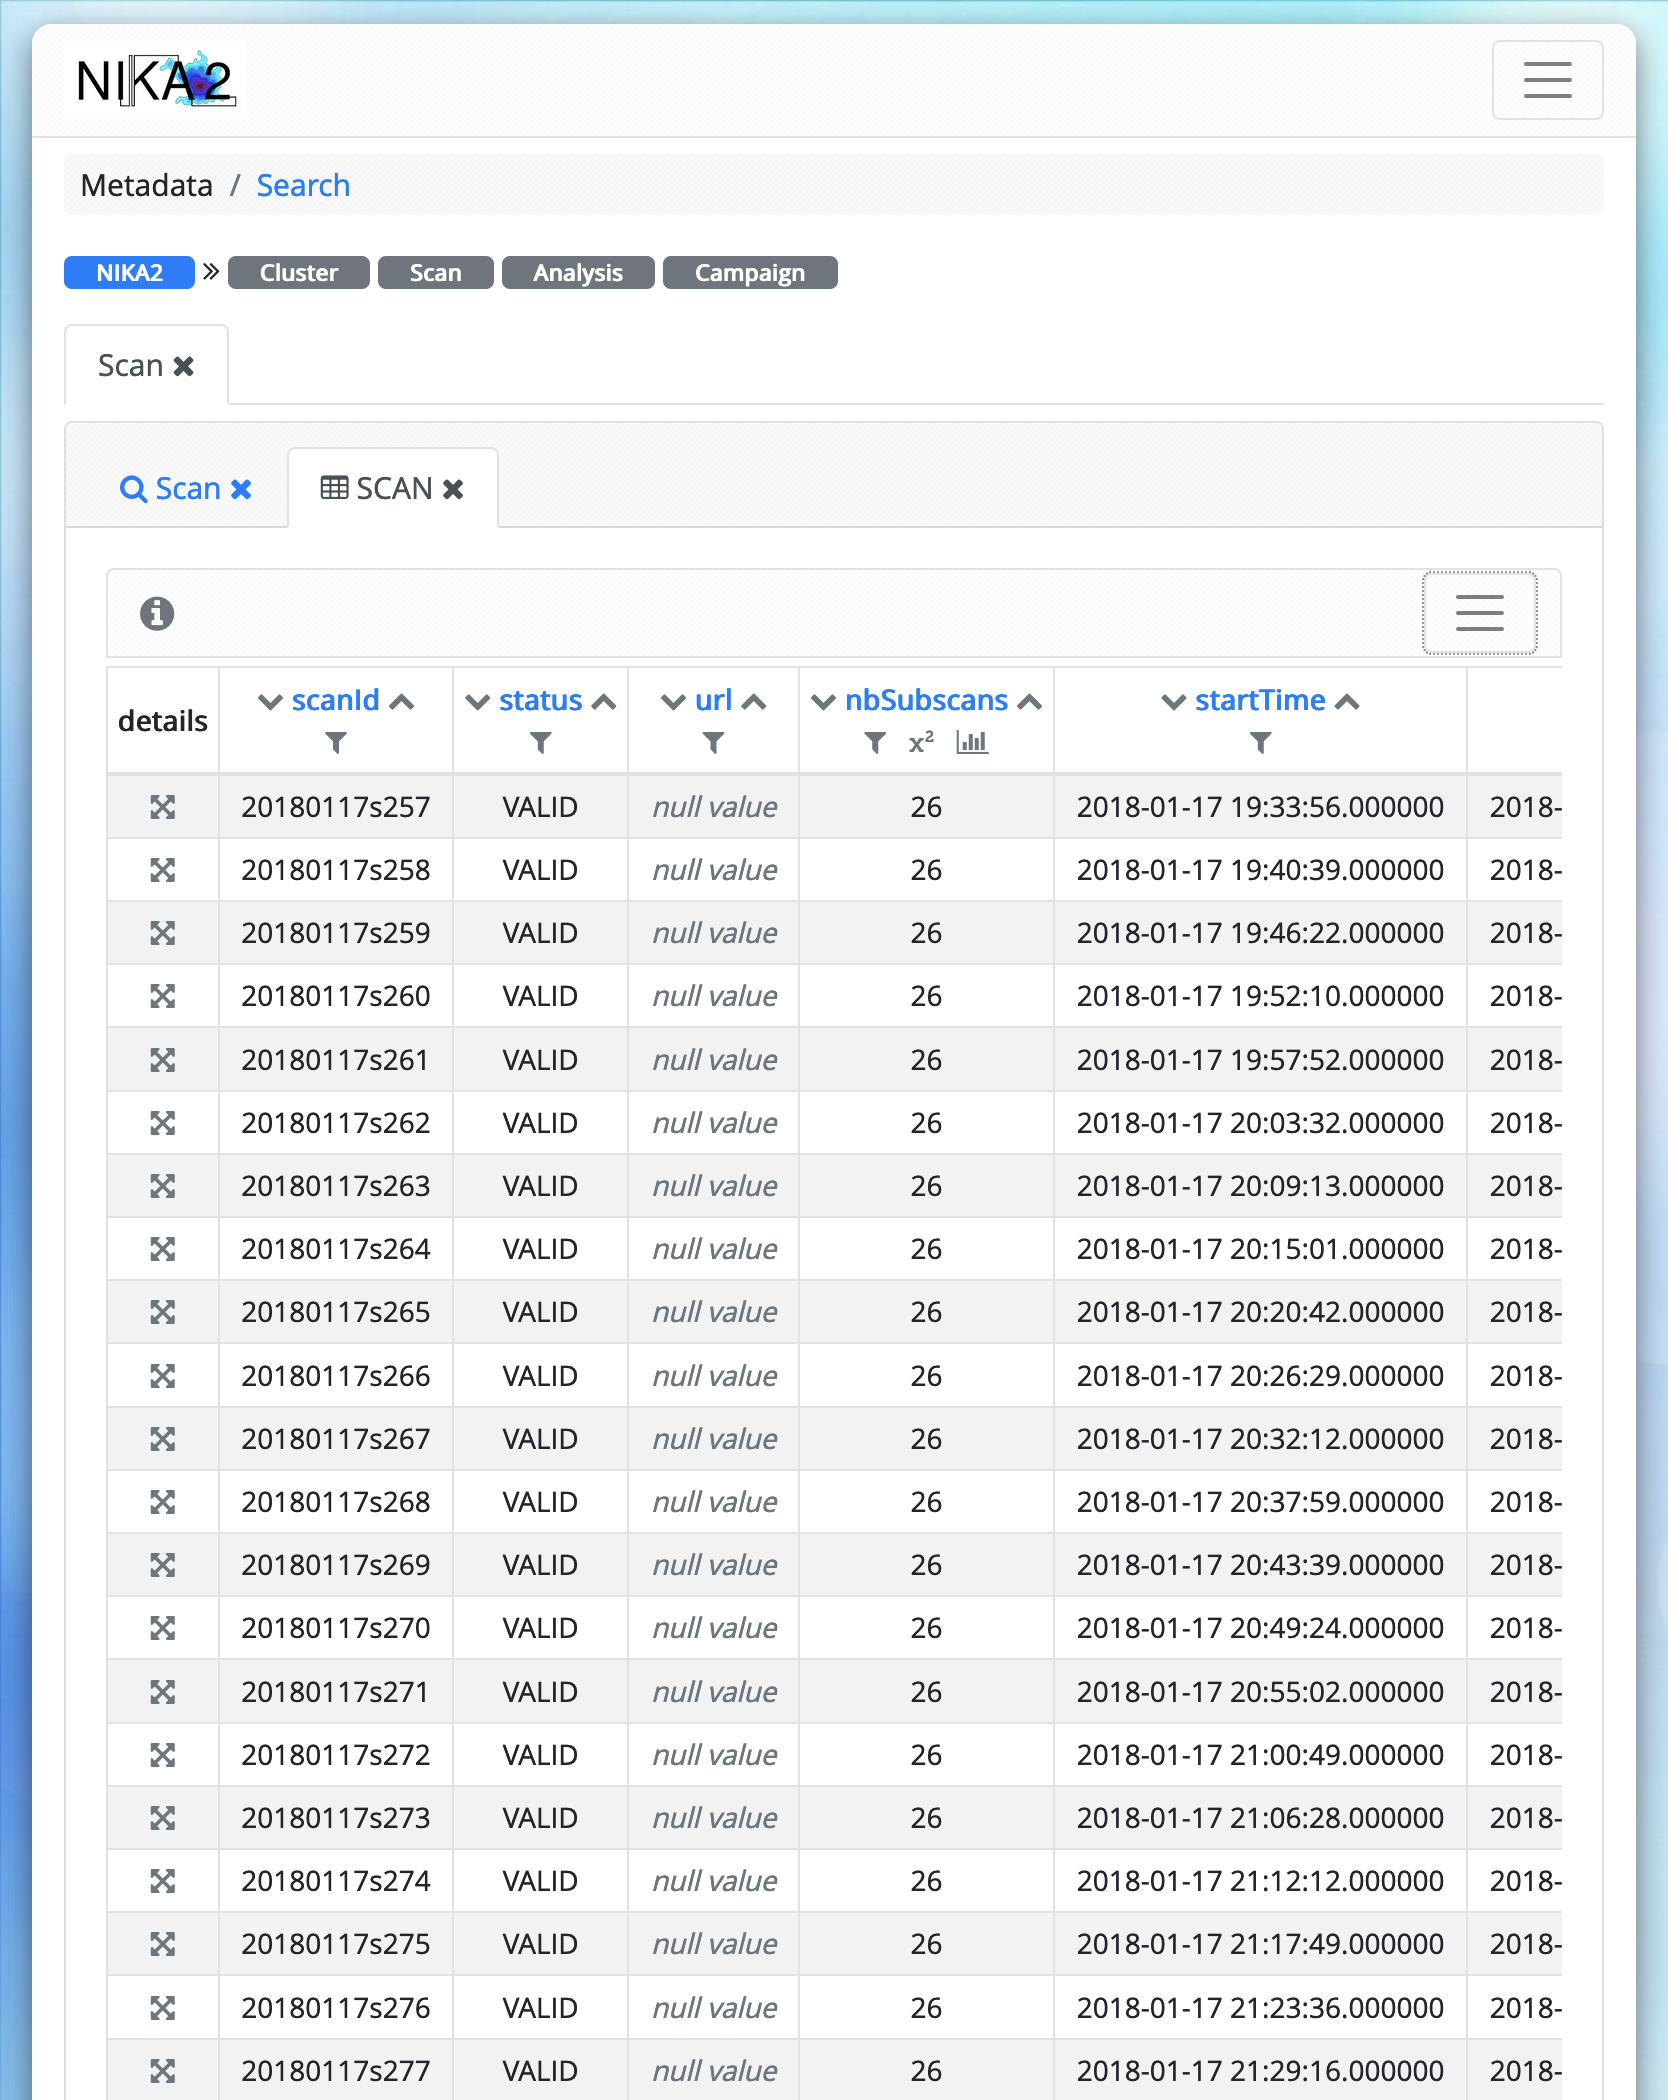
\includegraphics[width=.49\linewidth, trim={0 12cm 0 0}, clip]{Figures/Chap_nk/ami_results_2.png}
    \caption{
        Deux exemples de requêtes dans l'interface graphique de AMI (\textit{haut}) et leurs résultats (\textit{bas}).
        \textbf{Gauche:} recherche des amas du grand programme SZ dont le redshift est compris entre 0.5 et 0.7.
        \textbf{Droite:} recherche des \textit{scans} de l'amas \act\ ayant été effectués pour une opacité atmosphérique $\tau_{225}$ entre 0.1 et 0.2.
    }
    \label{fig:ami_request}
\end{figure*}

La base de données peut également être interrogée en Python.
Cette fonctionnalité est particulièrement intéressante pour interfacer les logiciels de traitement de données du grand programme SZ avec la base de données AMI-LPSZ.
Par exemple, le traitement des données brutes de NIKA2 décrit au chapitre \ref{chap:decorr} nécessite de connaître la liste des \textit{scans} associés à l'amas considéré.
Cette liste est facilement accessible grâce à l'interface Python, ce qui simplifie grandement le processus.
Il est également possible d'utiliser cette interface pour créer automatiquement les fichiers nécessaires pour les observations au télescope.

% ------------------------------------------------------------------------------------- %
\subsection{Développements futurs}

La base de données AMI-LPSZ offre un grand nombre de fonctionnalités qui ont déjà énormément facilité la gestion du grand programme SZ.
Certains aspects restent cependant à développer.
L'un des objectifs serait de stocker dans AMI les résultats des différentes étapes de l'analyse des données de chaque amas, de l'analyse des données brutes décrite au chapitre \ref{chap:decorr} aux propriétés thermodynamiques traitées au chapitre \ref{chap:panco}.
Pour l'instant, les résultats d'analyse ne sont pas stockés sur la base de données, car la structure des métadonnées à y sauvegarder n'a pas été définie.
De plus, la gestion des données externes est pour l'instant sommaire.
L'information sur ces données est consignée dans un champ correspondant à un dictionnaire clé-valeur pour chaque amas.
Dans ce champ, chaque clé indique le nom d'un instrument (\textit{XMM-Newton} ou \textit{Chandra} pour les observations X, SPIRE, PACS ou FIRST pour les sources ponctuelles, etc), et la valeur associée est un booléen, indiquant l'existence ou non de données correspondant à chaque instrument.
Un objectif de la base de donnée serait de compléter ces champs avec plus d'information, par exemple l'adresse à laquelle les données peuvent être récupérées.
Cette base de données représente donc un outil déjà extrêmement utile pour le grand programme SZ de NIKA2, mais qui pourra le devenir encore plus avec une définition de la structure des données pertinentes à stocker pour les données externes et les résultats d'analyse.
